%%% File encoding: UTF-8

%%% Magic comments for setting the correct parameters in compatible IDEs
% !TeX encoding = utf8
% !TeX program = pdflatex 
% !TeX spellcheck = de_DE
% !BIB program = biber

\RequirePackage[utf8]{inputenc} % Remove when using lualatex or xelatex!
\RequirePackage{hgbpdfa}        % Creates a PDF/A-2b compliant document

\documentclass[bachelor,english,smartquotes]{hgbthesis}
% Valid options in [..]: 
%    Type of work: 'diploma', 'master' (default), 'bachelor', 'internship' 
%		 Additionally for a thesis exposé: 'proposal (for 'bachelor' and 'master')
%    Main language: 'german' (default), 'english'
%    Turn on smart quote handling: 'smartquotes'
%    APA bibliography style: 'apa'
%%%-----------------------------------------------------------------------------

\usepackage[printonlyused]{acronym}
\usepackage{hyperref}
\usepackage{subfig}
\usepackage{booktabs}
\usepackage{rotating}
\usepackage{array}

\graphicspath{{images/}}  % Location of images and graphics
\logofile{logo}           % Logo file: images/logo.pdf (no logo: \logofile{})
\bibliography{references} % Biblatex bibliography file (references.bib)

%%%-----------------------------------------------------------------------------
\begin{document}
%%%-----------------------------------------------------------------------------

%%%-----------------------------------------------------------------------------
% Title page entries
%%%-----------------------------------------------------------------------------

\title{Location-Based Alerts for Passengers \\ in Public Transportation}
\author{Antonia\ Stieger}
\programname{Mobile Computing}

\programtype{Fachhochschul-Bachelorstudiengang} % select/edit
%\programtype{Fachhochschul-Masterstudiengang}

\placeofstudy{Hagenberg}
\dateofsubmission{2025}{03}{15} % {YYYY}{MM}{DD}

\advisor{FH-Prof. Dr.-Ing. Jens~Kr\"osche}

%\strictlicense % restrictive license instead of Creative Commons (discouraged!)

%%%-----------------------------------------------------------------------------
\frontmatter                                   % Front part (roman page numbers)
%%%-----------------------------------------------------------------------------

\maketitle
\tableofcontents

% \include{front/preface} % A preface is optional
\chapter{Abstract}

%The main objective of this paper was to analyse comprehensively the urban public transport usage, satisfaction levels and the satisfaction impact on usage of public transport in European Union (EU) countries.

This should be a 1-page (maximum) summary of your work in English.

		
\include{front/kurzfassung}			

%%%-----------------------------------------------------------------------------
\mainmatter                                    % Main part (arabic page numbers)
%%%-----------------------------------------------------------------------------

\chapter{Introduction}
\label{cha:Introduction}

\section{Motivation}

\section{Problem definition}

\section{Definition of goals}

\section{Structure of thesis}


% 1. Location-Based Alerts for Passengers in Public Transport
% 2. Optimizing Public Transit with Geofencing Stop Alerts
% 3. Geofencing Alerts to Enhance Passenger Awareness of Stops

% 4. The Role of Geofencing in Public Transportation Stop Alerts
% 5. Enhancing Passenger Experience in Public Transit: Effective Stop Reminder Systems
% 6. The Role of Stop Reminder Solutions in Public Transport
% 7. Enhancing Passenger Awareness with Stop Alerts in Public Transport

\chapter{Fundamentals}
\label{cha:Fundamentals}

This chapter provides an overview of the core concepts relevant to the thesis. It begins by reviewing various positioning methods as well as systems for indoor and outdoor settings, followed by an examination of how smartphones handle alerts, including different types and influencing factors in iOS. Geofencing technologies are analyzed for their functionality, use cases and limitations. Finally, advancements in technologies such as speech-to-text and large language models are discussed in the context of voice-controlled reminder systems.

\section{Positioning Methods}
\label{sec:methods}
The term "positioning" refers to the ability to determine an object's location within a defined space. According to K\"upper \cite{kupper2005location}, positioning relies on the measurement of observables, which describe the spatial relationship between a target and its reference points. Depending on the positioning technology used, observables can include angles, ranges, range differences or velocity and they are measured by analyzing the properties of pilot signals. 
Pilot signals, such as radio, infrared or ultrasound signals, are reference signals transmitted from a known source and by identifying their origin, a fixed point with known coordinates, the position of the target can be calculated using positioning techniques. These techniques vary based on the type of observable measured and include proximity sensing, lateration, angulation, pattern matching and inertial navigation.
The computed position is expressed relative to a chosen reference system. This system could be descriptive, such as identifying a specific cell in a grid, or geodetic, where the position is represented as two- or three-dimensional coordinates based on WGS-84 or UTM. Further details on the different positioning techniques are provided in the following sections.

\subsection{Proximity Sensing}
Proximity sensing, as described by K\"upper \cite{kupper2005location}, is the simplest positioning method.
It works by leveraging the limited coverage range of pilot signals to detect the presence or absence of a terminal within a specific area. 
In this context, a terminal refers to a device or object whose position is being determined, such as a mobile or IoT device.
Due to the limited range of these pilot signals, the terminal's position is assumed to correspond to the location of the base station communicating with it.
Militaru et al. \cite{militaru2024positioning} illustrate the concept of proximity sensing in Fig.~\ref{fig:proximity2}.

\begin{figure}[htbp]
    \centering
    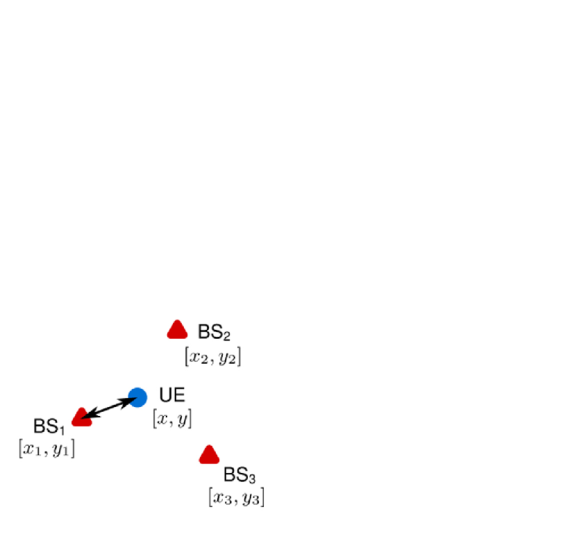
\includegraphics[width=0.4\textwidth]{proximity2.pdf}
    \caption{Proximity sensing \cite{militaru2024positioning}}
    \label{fig:proximity2}
\end{figure}

In the words of K\"upper \cite{kupper2005location}, proximity sensing in cellular networks is often referred to as \ac{CoO}, Cell Global Identity or Cell-ID. 
A "cell" is a geographic area within the cellular network, managed by a base station that serves as a local signal hub for devices within that area. 
The accuracy of the location determined through \acs{CoO} depends largely on the size and shape of the cell, as highlighted by Grejner-Brzezinska and Kealy \cite{grejner2004positioning} and Lee et al. \cite{lee2014localization}.
Smaller cells allow for better location estimates, often reaching accuracy within 100 meters in urban areas where cell towers are densely placed.
In rural areas, where cell coverage spans several kilometers, the location estimate becomes less accurate.

\acs{CoO} is considered an inexpensive solution, as noted by Grejner-Brzezinska and Kealy \cite{grejner2004positioning} and K\"upper \cite{kupper2005location}, because it is compatible with the existing infrastructure. 
A terminal can determine its location using \acs{CoO} either through an active connection to a base station or by passively receiving broadcast signals while in an idle state. 
When actively connected, the terminal's location is identified using the coordinates of the serving base station. 
In idle mode, the terminal can either query a remote database to retrieve the base station's location using its cell ID or rely on the base station to include its location directly in the broadcast signal, reducing the need for external lookups. 

\subsection{Lateration}
Lateration, the most widely used method for localization according to Lee et al. \cite{lee2014localization}, determines a target's location by measuring distances or distance differences from multiple reference stations. 
These measurements are referred to as "pseudoranges" because they include errors that distort the true ranges. 
Common error sources in lateration include clock errors, atmospheric effects or multipath propagation.
To determine a position, measurements from at least three stations are required.
Lateration techniques are categorized into circular lateration, which relies on absolute distance measurements and hyperbolic lateration, which uses differences in these distances across stations.

\subsubsection{Circular Lateration}
Circular lateration uses distance measurements to multiple base stations to derive a location. 
Assuming the base stations are at the same elevation, knowing the distance between the target and a single base station places the target somewhere on a circle centered on that station. 
Introducing a second base station allows for two possible positions where the two circles intersect. 
Adding a third base station resolves this uncertainty, pinpointing the target's exact location at the single intersection point of all three circles, according to K\"upper \cite{kupper2005location}. 
This process, known as trilateration, utilizes the Pythagorean theorem for calculations and is illustrated in Fig.~\ref{fig:circular_lateration} (a).

In three-dimensional space, each distance measurement defines a sphere around a base station. 
Kolodziej and Hjelm \cite{kolodziej2017local} note that with only three base stations, the target's position is narrowed down to two possible points where the spheres intersect. 
Typically, one of these points can be dismissed as implausible, such as a location in outer space. 
To eliminate any ambiguity, a fourth base station is introduced as can be seen in Fig.~\ref{fig:circular_lateration} (b), ensuring a unique position fix. Additionally, the fourth base station is necessary in synchronizing clocks.
% Positioning methods based on circular lateration in combination with timing measure- ments are usually subsumed under the term Time of Arrival (ToA). GPS is the most prominent example where this method is applied. A GPS receiver determines pseudoranges to at least three satellites and calculates its position from that. For clock synchronization between receiver and satellite, it is usually required to observe the signals from a fourth satellite. This will be explained in Chapter 7 in detail
% Küpper:As can be derived from this figure, range measurements must be made to at least four satellites, three for obtaining the position in 3D and the other for time synchronization between the satellites and the receiver. As GPS applies circular lateration, it requires very exact time synchronization (see Section 6.2.2.1). 

\begin{figure}[htbp]%
    \centering
    \subfloat[\centering]{{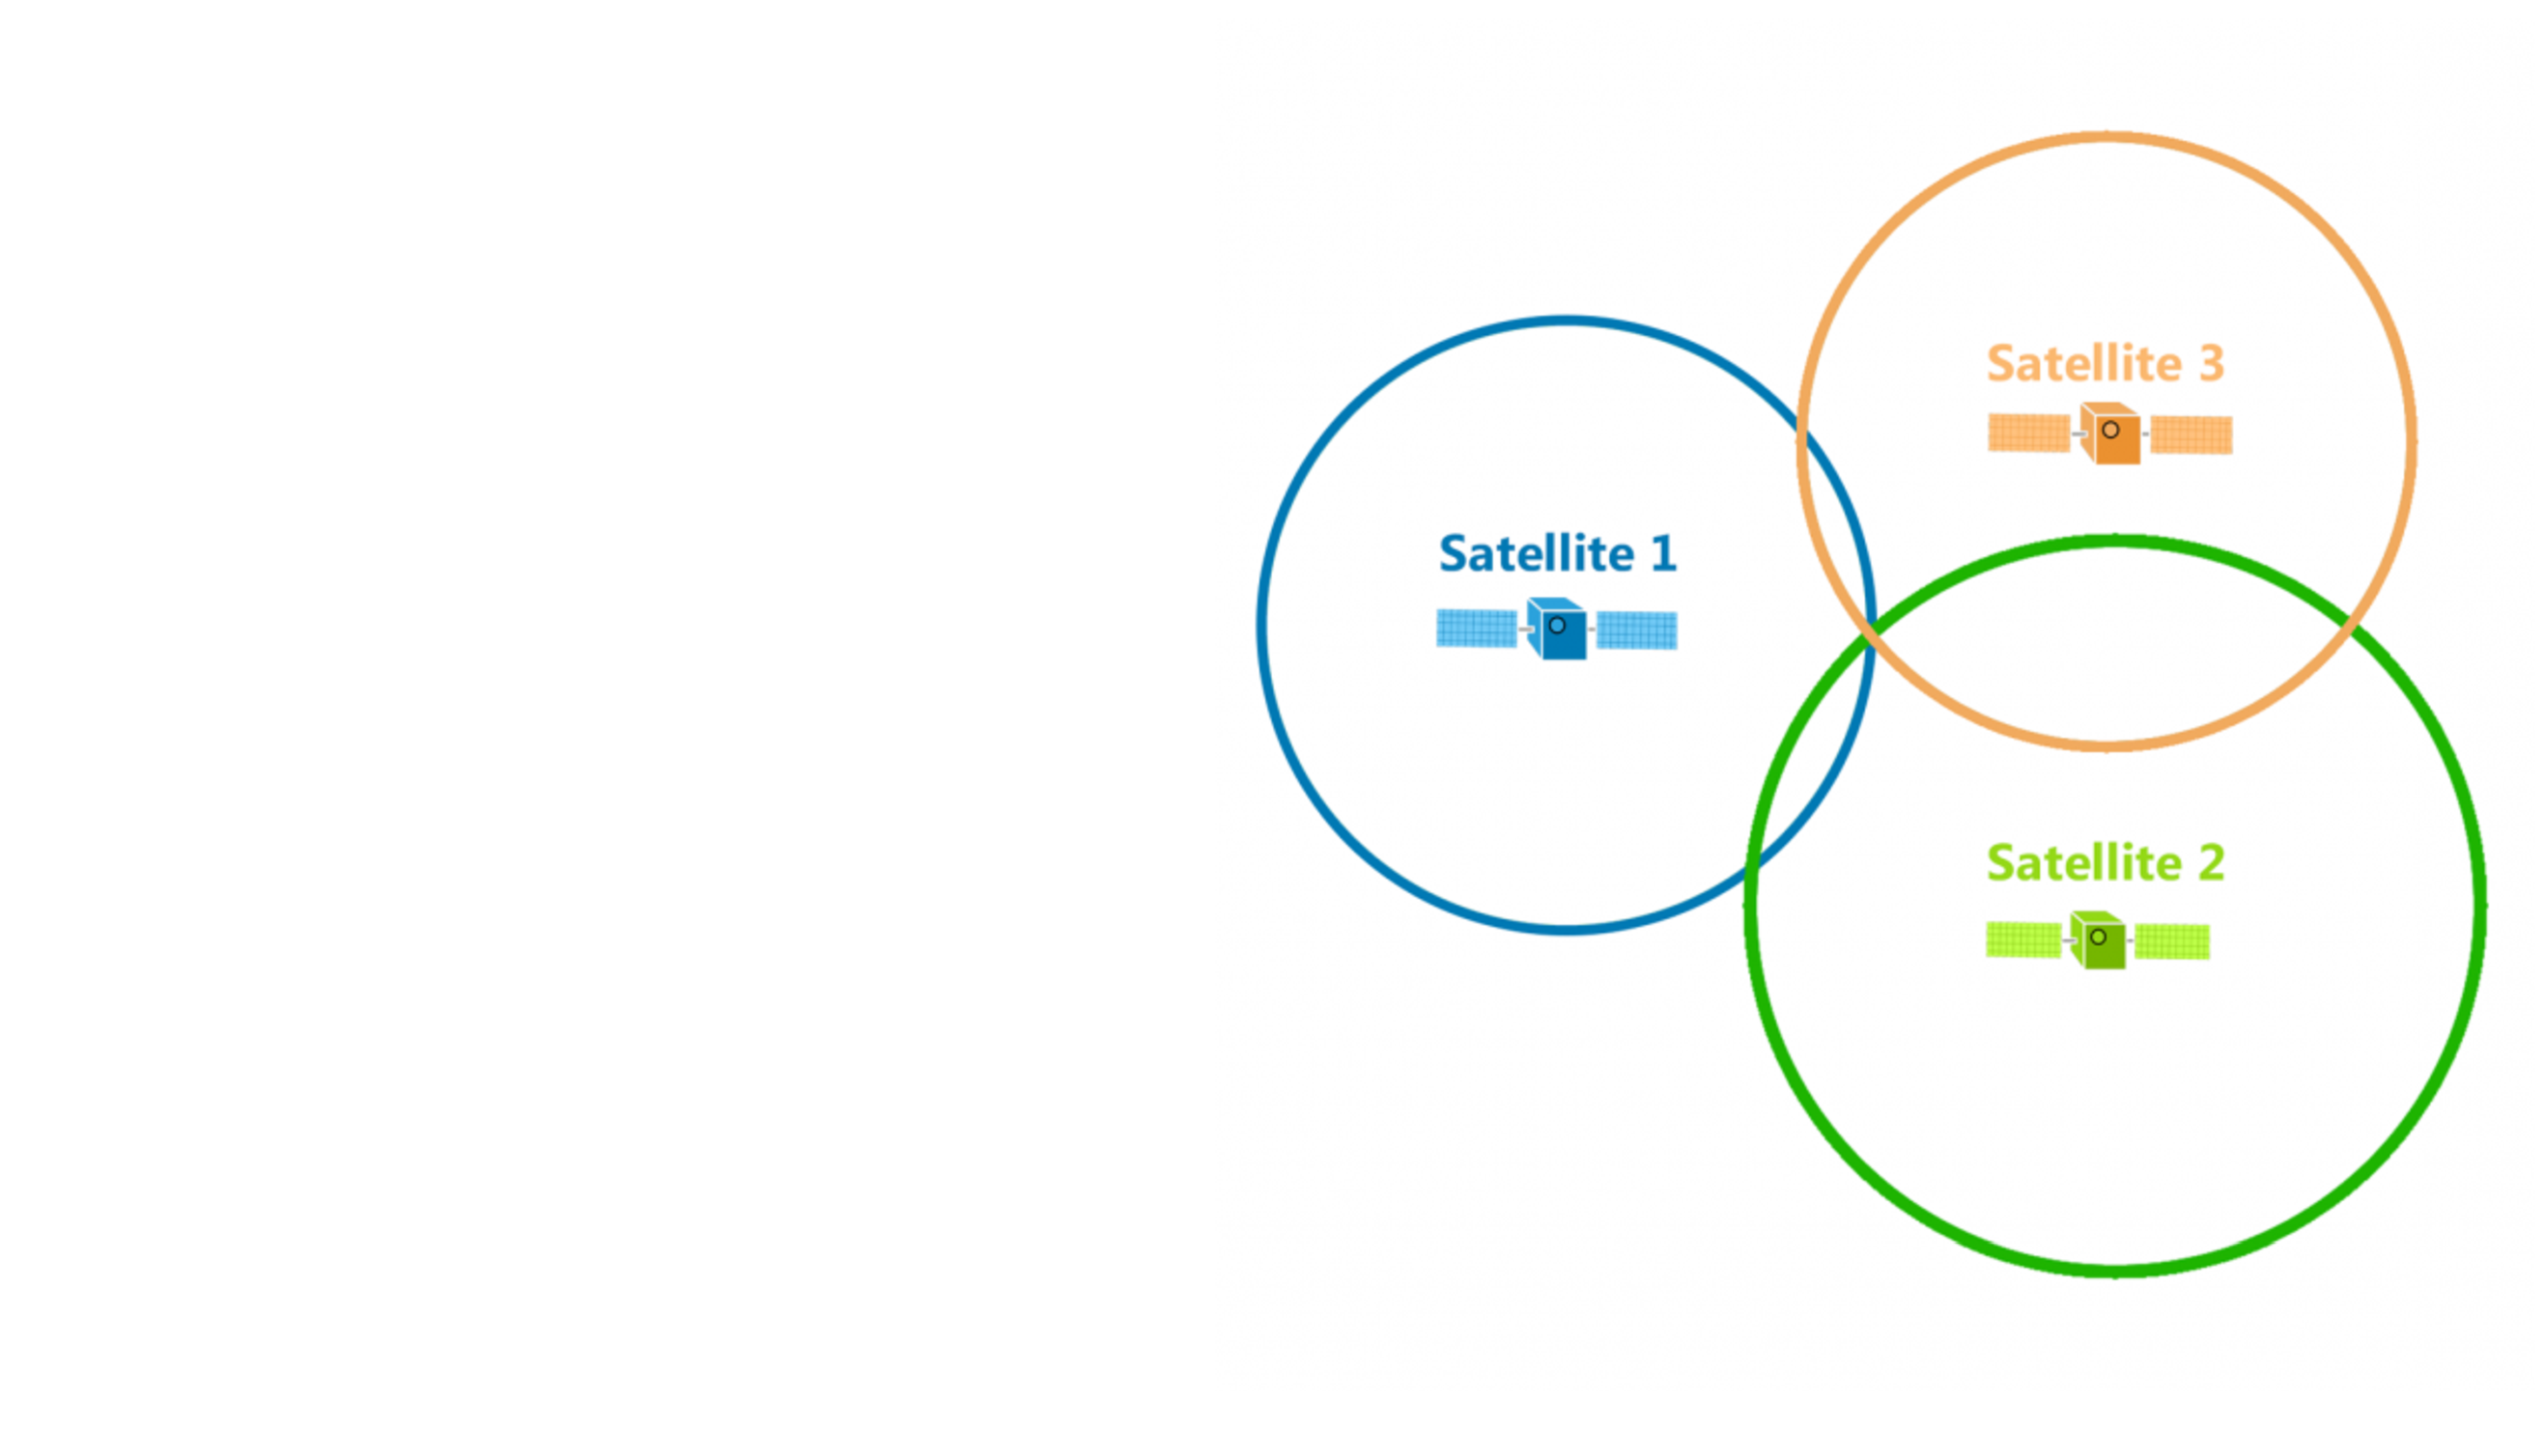
\includegraphics[width=5cm]{lateration_2d.pdf}}}%
    \qquad
    \subfloat[\centering]{{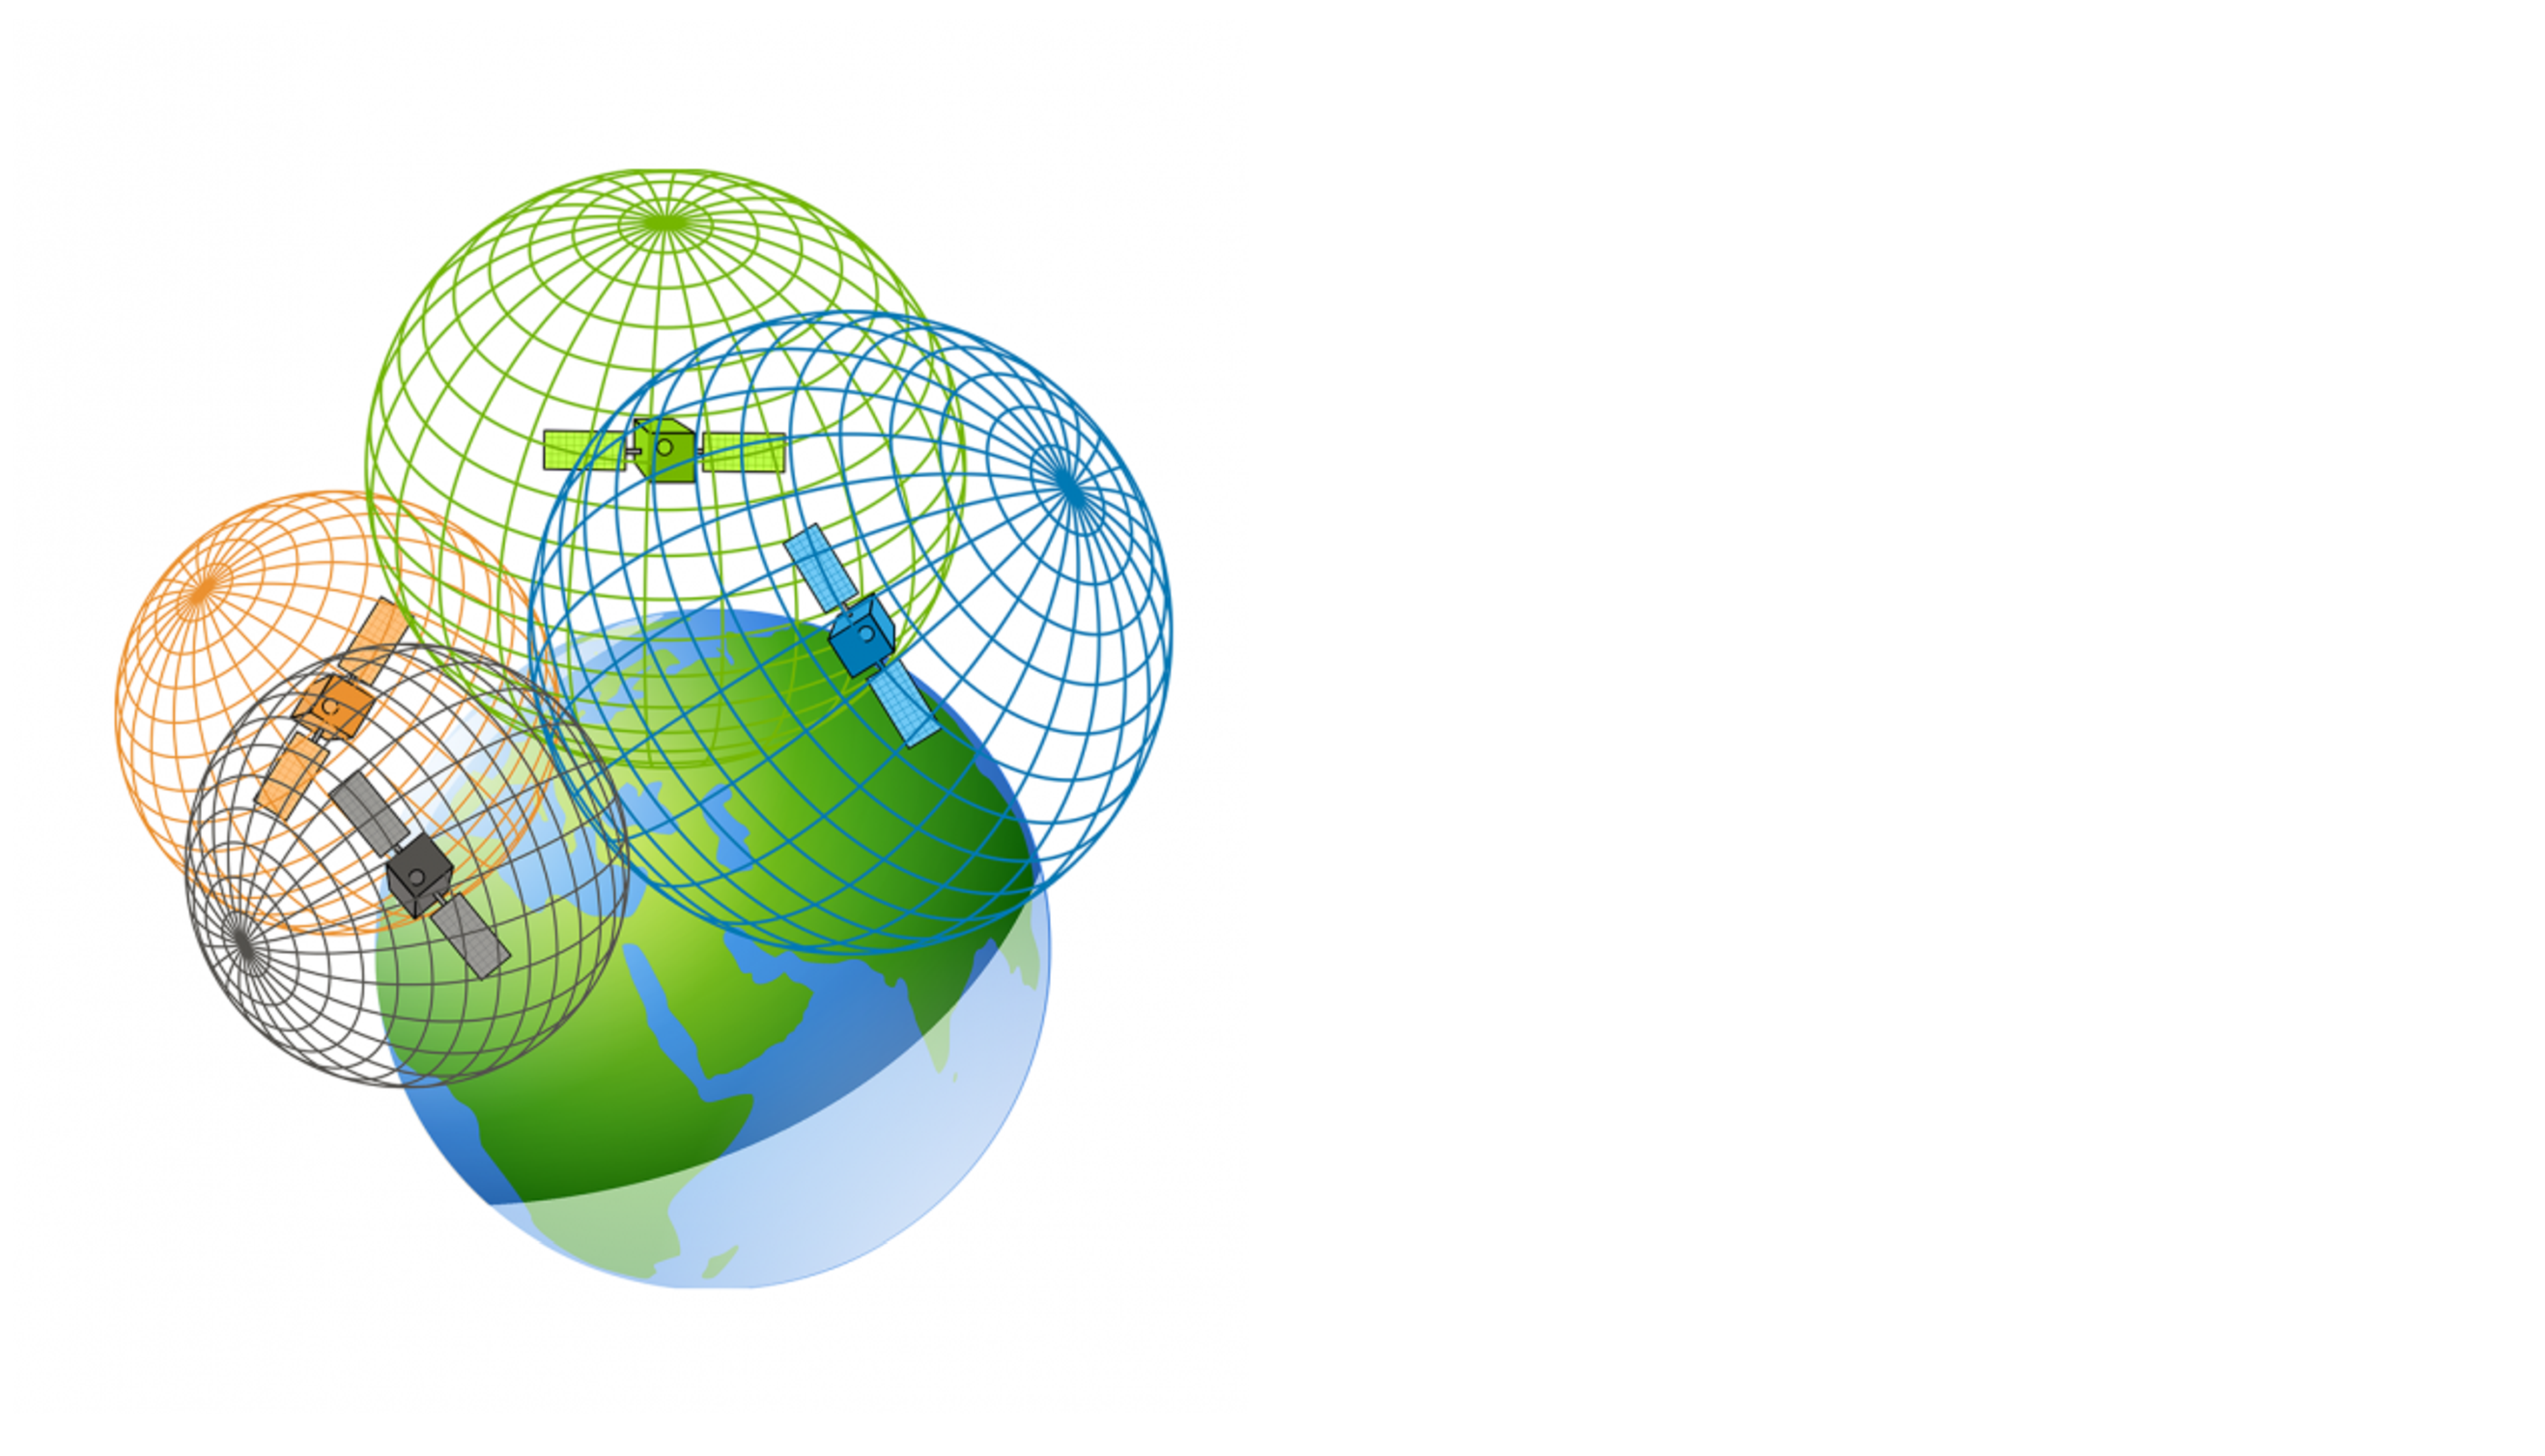
\includegraphics[width=5cm]{lateration_3D.pdf}}}%
    \caption{Circular lateration with three (a) and four (b) base stations (satellites) \cite{gisgeography_trilateration}}%
    \label{fig:circular_lateration}%
\end{figure}

\subsubsection{Hyperbolic Lateration}
In contrast to circular lateration, hyperbolic lateration determines a position by measuring differences in distance rather than absolute distances. 
A hyperbola represents all points that maintain a constant range difference relative to two fixed points. 
K\"upper \cite{kupper2005location} explains that with the known range difference between the target and two base stations, the target's possible locations are constrained along a hyperbolic path between them. 
This method, illustrated in Fig.~\ref{fig:hyperbolic_lateration} (a), uses two base stations to determine a single hyperbolic path. 
However, with just two base stations, the target's precise location cannot be unambiguously determined, as it could lie anywhere along the hyperbola.
To resolve this ambiguity, a third base station is introduced, as shown in Fig.~\ref{fig:hyperbolic_lateration} (b). By adding this third base station, a second hyperbola is created and the target's position is estimated at the intersection of these two hyperbolas. 
In three-dimensional space, the principle extends to hyperboloids, requiring at least three base stations for an unambiguous position fix.
A key advantage of hyperbolic lateration, according to Werner \cite{werner2014indoor}, is that it only requires synchronization among the base stations' clocks, rather than between the stations and the target, because it relies on \ac{TDoA} measurements. 
With \acs{TDoA}, only the relative arrival times at the base stations matter, making the exact emission time from the target irrelevant, as it is the same for all signals and cancels out in the calculation.

\begin{figure}[htbp]
    \centering
    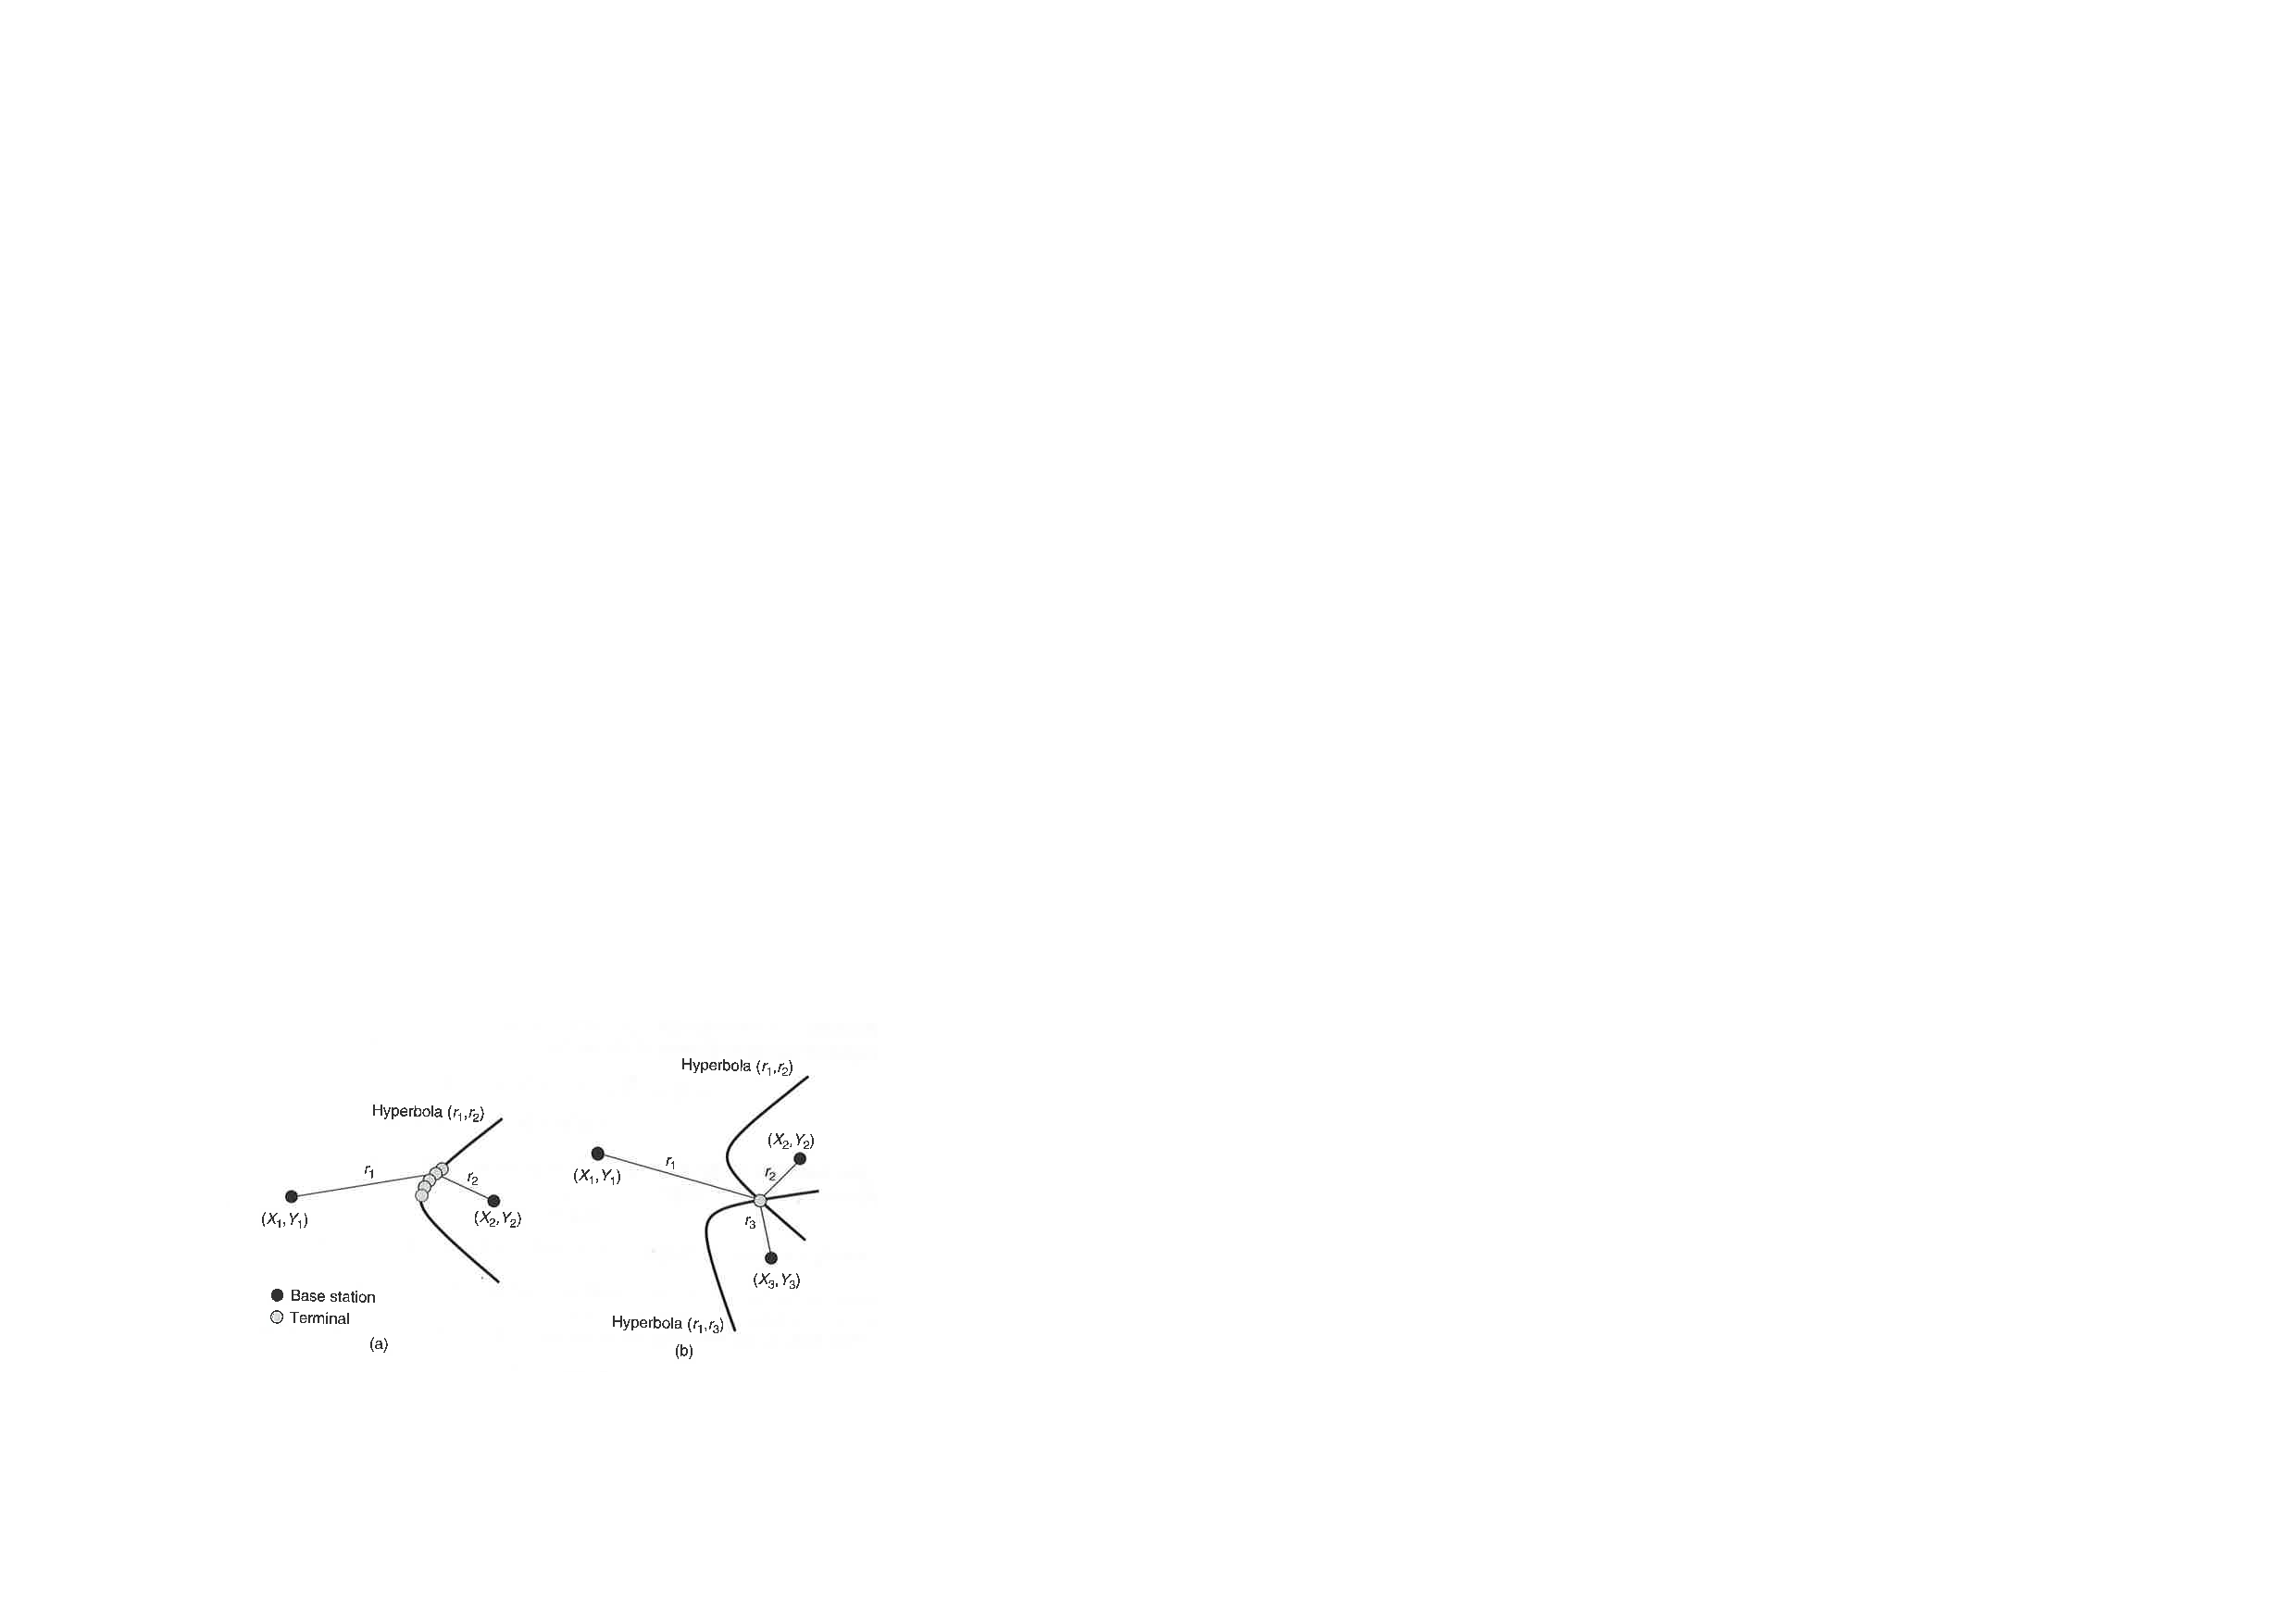
\includegraphics[width=0.7\textwidth]{hyperbolic_lateration.pdf}
    \caption{Hyperbolic lateration with two (a) and three (b) base stations \cite{kupper2005location}}
    \label{fig:hyperbolic_lateration}
\end{figure}

\subsection{Angulation}
Angulation is a positioning technique that determines an object's location based on the angles at which signals are received from multiple reference points, rather than measuring distances. 
According to K\"upper \cite{kupper2005location} it is also called \ac{AoA} or \ac{DoA}. 
To determine the angle of incoming pilot signals, either the base station or the terminal must be equipped with antenna arrays.
However, K\"upper \cite{kupper2005location} highlights that angulation is predominantly used as a network-based method today, meaning that the arrays are more commonly installed at the base station rather than the terminal due to cost and complexity considerations.
Once the angles from at least two base stations are known, the object's position can be determined by plotting lines along these angles, the point where the lines intersect reveals the target's location. 

Technically, two angle measurements are sufficient to determine a position in 2D, but angulation is sensitive to errors caused by the resolution of antenna arrays, which can lead to approximations of the actual angle rather than precise measurements.
These errors increase when the target is farther from the base station, making measurements less reliable at long distances.
Additionally, in non-line-of-sight conditions, multipath propagation introduces further inaccuracies as signals reflect off obstacles and arrive at the base station from unintended directions. 
To mitigate these errors, measurements from at least three base stations are recommended.
Fig.~\ref{fig:angulation2} illustrates how angle measurements from three base stations intersect to determine the terminal's position.

\begin{figure}[htbp]
    \centering
    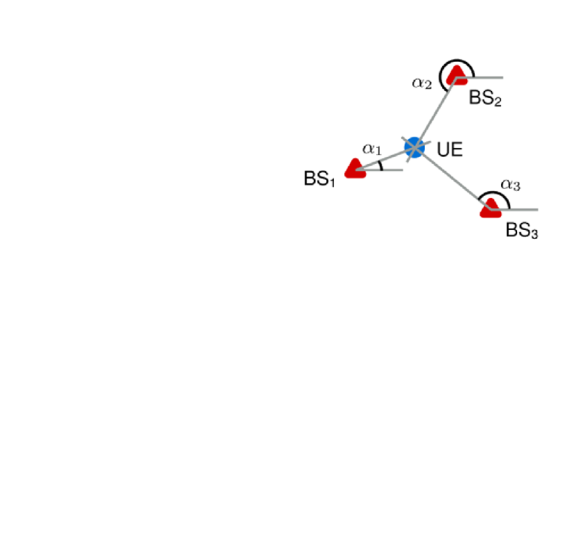
\includegraphics[width=0.4\textwidth]{angulation2.pdf}
    \caption{Angulation using three base stations \cite{militaru2024positioning}}
    \label{fig:angulation2}
\end{figure}

\subsection{Pattern Matching}
Pattern matching is a method of finding a target's position by observing its surroundings and identifying patterns in the environment to determine where it is.
K\"upper \cite{kupper2005location} divides the matching of a target pattern with a known reference into two types: optical and nonoptical pattern matching.

\subsubsection{Optical Pattern Matching}
Optical pattern matching, also known as scene analysis, determines the position of a target by capturing and comparing images of a scene using a camera.
This method can be categorized into two types: static and dynamic scene analysis, as described by Küpper \cite{kupper2005location}.
In static scene analysis, a single image of the scene is compared to a database of pre-recorded images taken from various positions and angles. 
The target to be located could be the observer or another object within the scene. 
By matching the current image with the database, the target's position is identified.
Dynamic scene analysis, on the other hand, determines the target's position by analyzing changes between consecutive images captured over time. 

\subsubsection{Nonoptical Pattern Matching}
Nonoptical pattern matching identifies a target's position by analyzing measurable physical properties of the environment. 
When these properties are based on radio signal characteristics, the technique is commonly referred to as fingerprinting, as noted by Küpper \cite{kupper2005location} and Werner \cite{werner2014indoor}.

Fingerprinting is particularly effective for indoor positioning when combined with WLAN and consists of two main phases: the offline phase and the online phase. 
In the offline phase, the area is divided into a grid and at each grid point, \ac{RSS} from nearby base stations are recorded. 
These measurements create unique "fingerprints" that are stored in a database, each linked to its respective grid location.
During the online phase, the terminal collects \acs{RSS} values at its current location to form a sample vector. This vector is then transmitted to a server, which compares it with the database of fingerprints recorded during the offline phase. 
By identifying the closest match, the system estimates the target's position.
K\"upper \cite{kupper2005location} further explains that the matching process often utilizes algorithms like calculating Euclidean distances between signal vectors, though advanced methods like neural networks or Bayesian models can also be applied.

\subsection{Inertial Navigation}
Inertial navigation approximately calculates the current position by starting from a known location and using measurements of direction, velocity and time to compute the path traveled.
This method represents a modern approach to dead reckoning, which was widely used by explorers during the Middle Ages. 
They navigated using tools such as compasses, log lines and estimates of speed and time, as detailed by Taylor \cite{taylor1950deadreckoning}. 
Figure~\ref{fig:deadreckoning} illustrates this process of approximating position through dead reckoning.

\begin{figure}[htbp] 
    \centering 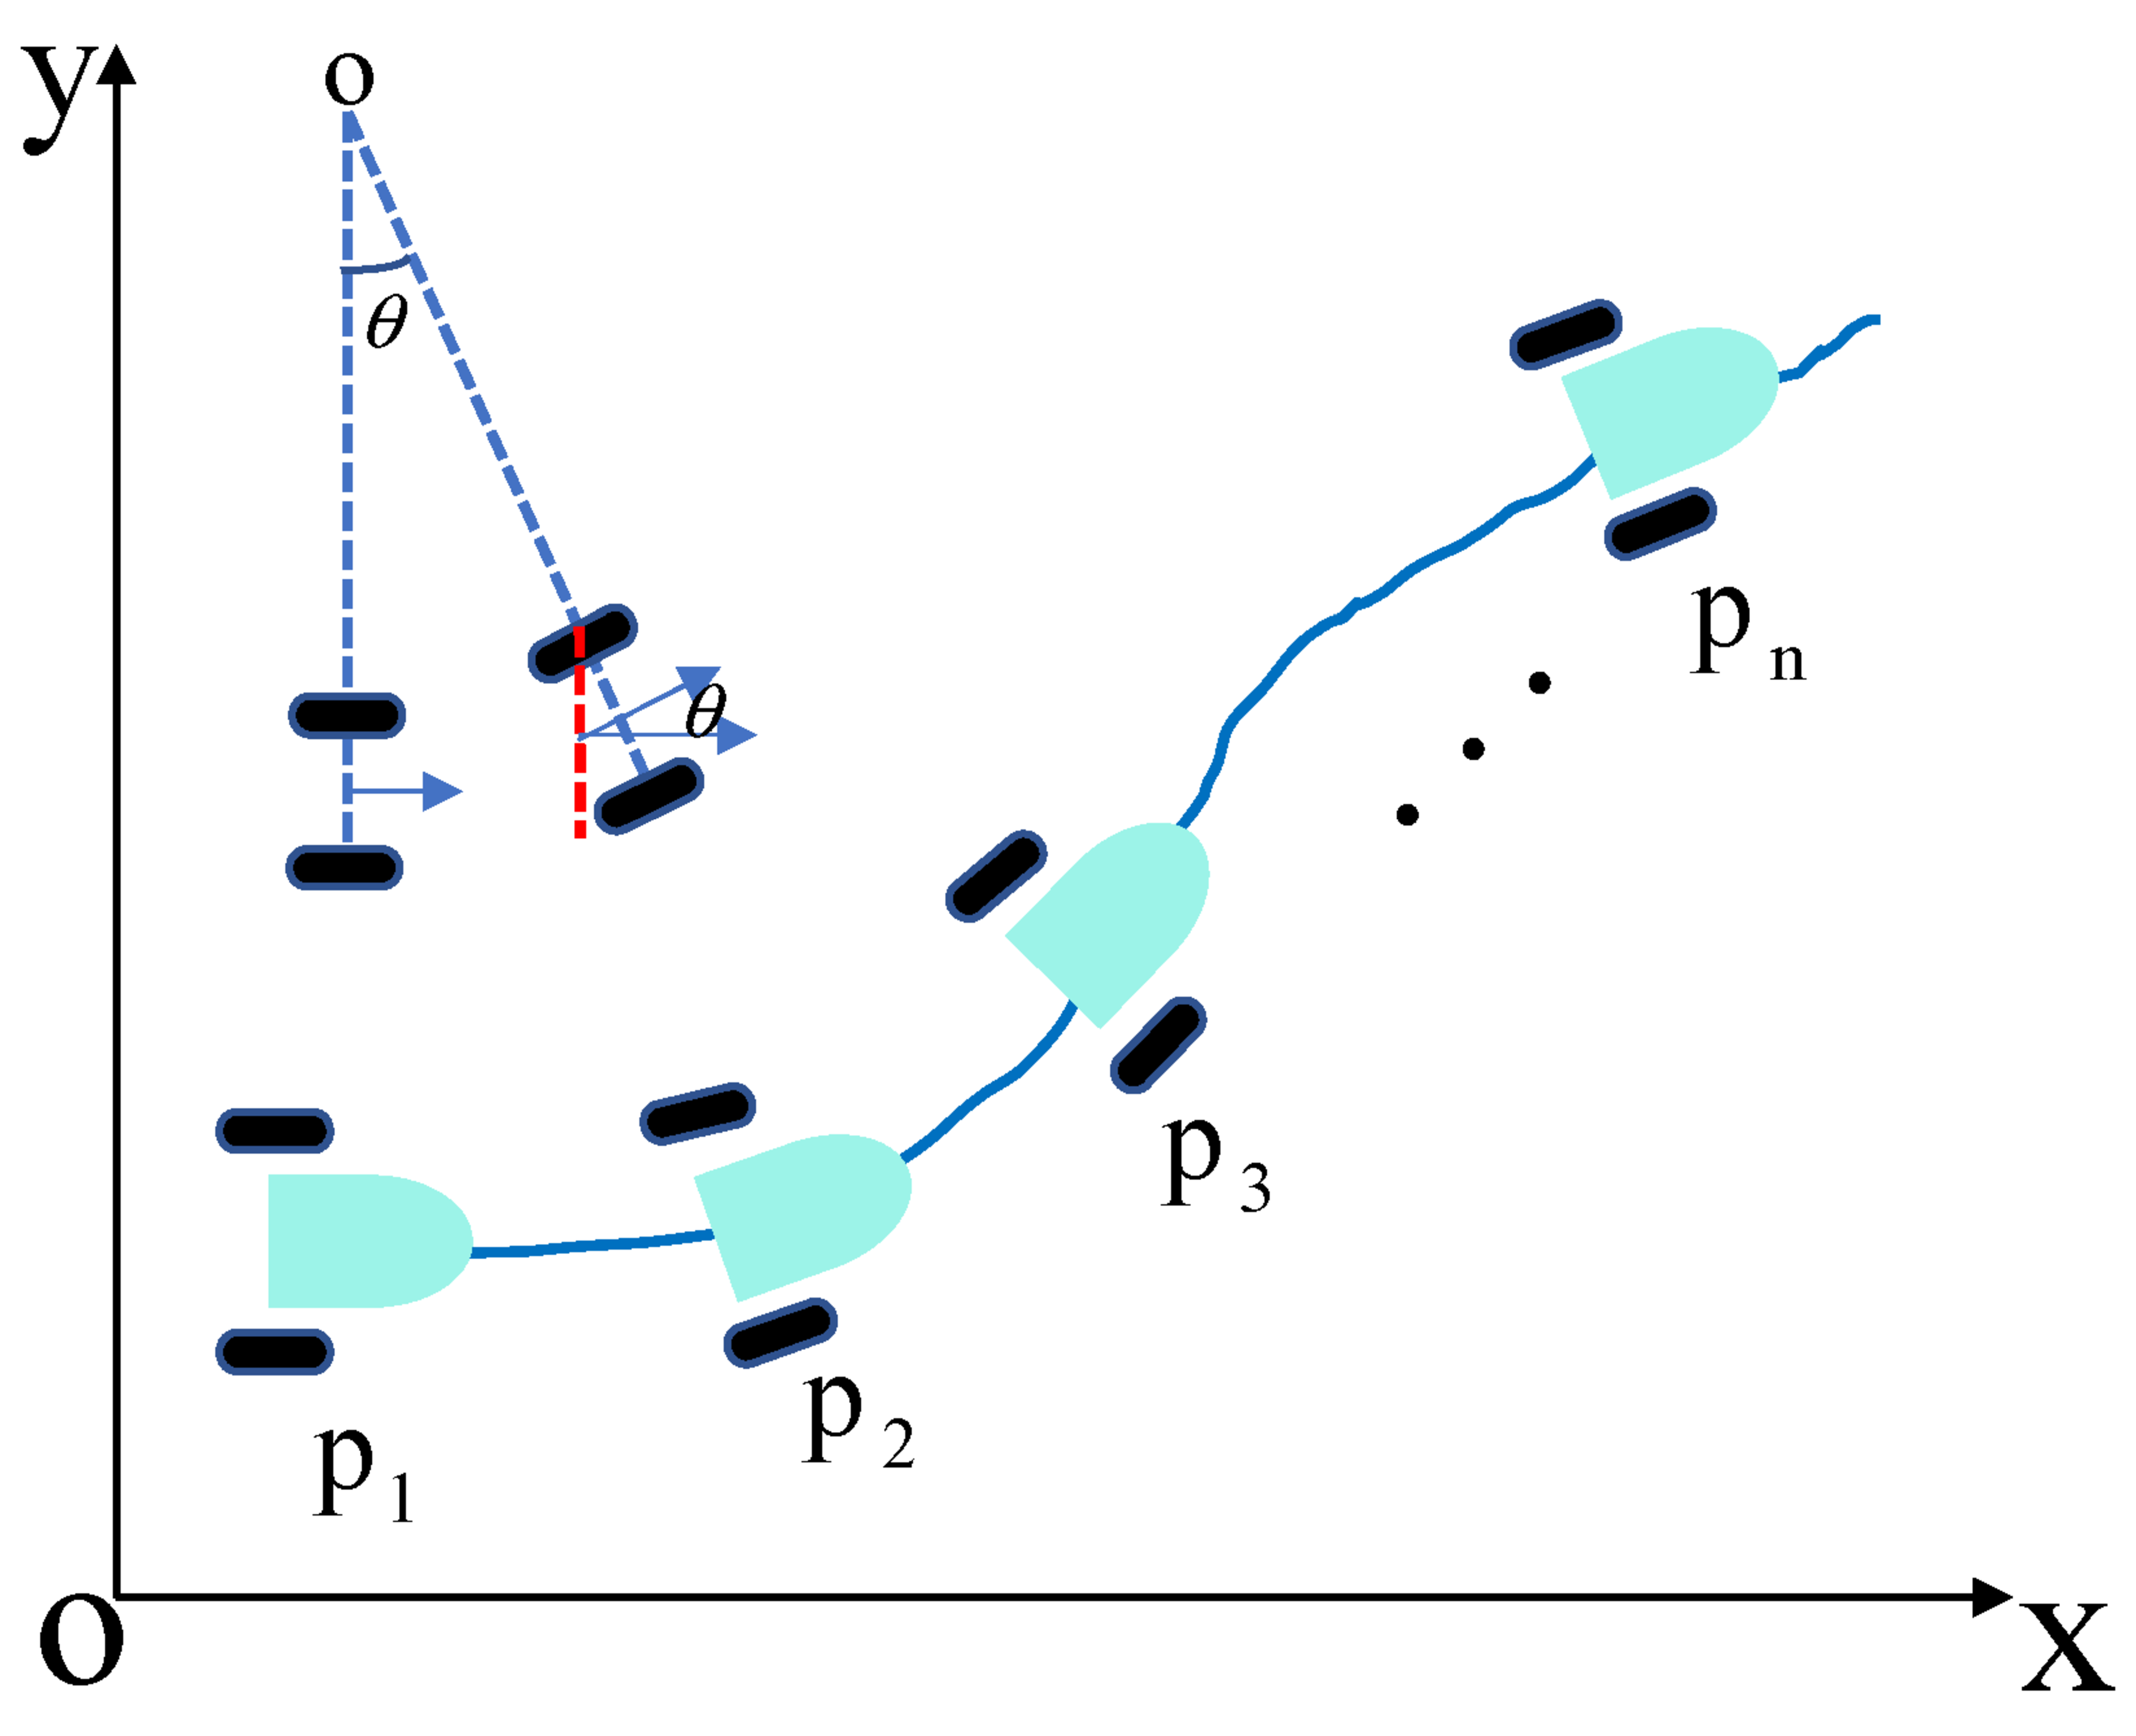
\includegraphics[width=0.5\textwidth]{deadreckoning.pdf} 
    \caption{Principle of dead reckoning \cite{wei2022positioning}} 
    \label{fig:deadreckoning} 
\end{figure}

While inertial navigation shares these conceptual roots, it leverages modern technology to measure motion far more precisely. 
An \ac{INS} relies on data from an \ac{IMU}, which contains accelerometers to measure linear acceleration and gyroscopes to track angular rotation. 
Once an initial position is established using methods like lateration or angulation, an \acs{INS} operates independently and doesn't rely on external electromagnetic signals like radio signals. 
This self-contained nature makes inertial navigation highly robust against signal obstructions and manipulation, but they still are highly susceptible to errors.
El-Sheimy \cite{sheimy2006ins} explains that position errors grow quadratically as a result of velocity errors that stem from biases or inaccuracies in accelerometer measurements during the initial integration process. 
He further points out that errors in gyroscopic data are even more impactful, as they first produce angular inaccuracies, which then propagate into velocity errors that grow quadratically and ultimately result in cubic error in position. 
These errors can accumulate over time due to the lack of external reference points. 
To mitigate this, inertial navigation is often only applied in short-term uses, such as to bridge periods when line-of-sight to satellites is obstructed or to refine position fixes determined by \ac{GNSS}, which is further discussed in Section \ref{sec:gnss}. 
By combining the last known location obtained via \acs{GNSS} with measurements captured by an \acs{IMU} chip, a vehicle's movement can still be tracked during GNSS outages, e.g. driving through a tunnel.

\subsection{Overview of Positioning Methods}
The previous sections have introduced a range of foundational positioning methods and to provide an overview, Table \ref{tab:table_methods} summarizes the key characteristics of the methods. 
The table is based on the works of K\"upper \cite{kupper2005location} and Werner \cite{werner2014indoor} and outlines the specific features each method observes, the tools and techniques used for measurement and the inherent limitations that may affect their performance.

\begin{table}[h!]
    \begin{center}
    \caption{Positioning methods in comparison}
    \label{tab:table_methods}
    \begin{tabular}{>{\centering\arraybackslash}p{4cm} >{\centering\arraybackslash}p{4cm} >{\centering\arraybackslash}p{5cm}}
        \toprule
        \textbf{Method} & \textbf{Observable} & \textbf{Measurement} \\
        \midrule
        Proximity Sensing & Physical proximity to a reference & Sensing pilot signals \\
        \addlinespace
        \hline
        \addlinespace
        Lateration & Distance and distance difference to reference point & Travel time and signal strength of pilot signals (or their differences) \\
        \addlinespace
        \hline
        \addlinespace
        Angulation & Angle to reference point & Antenna arrays \\
        \addlinespace
        \hline
        \addlinespace
        Pattern Matching & Comparison to reference patterns & Camera and received signal strength \\
        \addlinespace
        \hline
        \addlinespace
        Inertial Navigation & Acceleration, angular rotation and time from a reference & Accelerometers, gyroscopes and additional sensors depending on the infrastructure \\
        \addlinespace
        \bottomrule
    \end{tabular}
    \end{center}
\end{table}

\section{Positioning Systems}
As highlighted by K\"upper \cite{kupper2005location}, a target cannot determine its location on its own. 
Instead, it relies on a distributed infrastructure that implements positioning methods to compute its position. 
This infrastructure typically consists of components like base stations, which are fixed points with known coordinates, and terminals, whose positions are initially unknown. 
Depending on the type of system, satellite, cellular or indoor, the base stations may include satellites, cellular towers, \ac{WLAN} access points or tag readers. 
Terminals can range from mobile phones and laptops to vehicles and \ac{RFID} tags.
The components of such an infrastructure are depicted in Figure~\ref{fig:infrastructures}.

\begin{figure}[htbp] 
    \centering 
    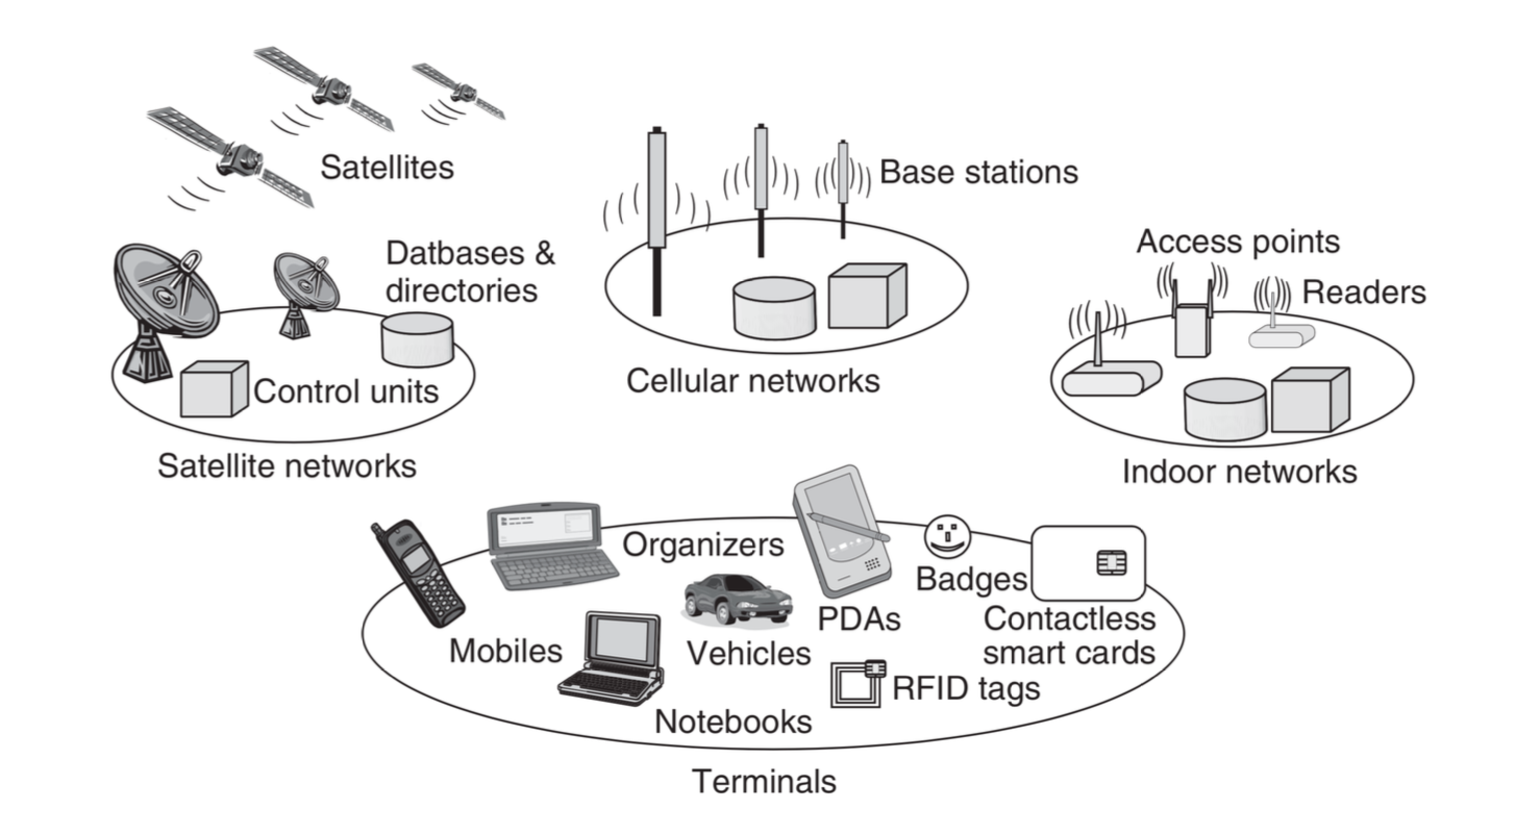
\includegraphics[width=0.8\textwidth]{infrastructures.pdf} 
    \caption{Infrastructures used in positioning \cite{kupper2005location}} 
    \label{fig:infrastructures} 
\end{figure}

In most cases, base stations either assist terminals in performing measurements or perform the measurements themselves. 
Additional components, such as databases and control units, may also be required for managing, processing and distributing positioning data. 
This section provides an overview of positioning systems, including cellular, \acs{GNSS}, \ac{Wi-Fi} and Bluetooth positioning systems, as well as inertial navigation systems, all of which rely on the positioning methods described in Section~\ref{sec:methods}.

% kolodziej2017local p. 106-107, 109-110
% werner2014indoor p. 88-98
% kupper2005location p. 91, 126-130, 155 (Satellite), 185 (Cellular), 233 (WLAN)

% In the area of transport and mobility positioning systems with their satellites in the orbit, such as GPS, GLONASS and Galileo, play a major role: They provide positioning services in outdoor environments and offer a way to compute one’s physical location on the globe. Besides the localization, outdoor positioning systems are also used in real- time navigation scenarios within car systems, navigation or mobile devices. Whether they are used for navigating home or to any other destination, they are an essential service of today’s life.
% While the above-mentioned positioning systems work great and reliable in outdoor environments, their performance and results are poor in indoor environments. Outdoor positioning systems such as GPS operate in direct line-of-sight scenarios with the satel- lites, which is not given indoors. As described by Jang and Kim [11], GPS signals cannot move easily through solid objects, as they get attenuated by e.g. walls. Moreover, the signals get reflected by the objects, which leads to inaccurate positioning results.
% To compensate the drawbacks of outdoor positioning systems in indoor scenarios, indoor positioning systems were developed to provide more reasonable results within buildings, but with the restriction to work only in specific indoor environments and not outside of its boundaries. Like outdoor positioning systems, they also provide means for localization and navigation, but within buildings using technologies such as Wi-Fi, Bluetooth, IR or cellular networks, as stated by Liu et al. [17].

% APPLE USES all available components on the device, including the Wi-Fi, GPS, Bluetooth, magnetometer, barometer, and cellular hardware 
%https://developer.apple.com/documentation/corelocation
%iOS and iPadOS devices might use Wi-Fi and Bluetooth to determine your location. GPS and cellular location are available on iPhone and iPad (Wi-Fi + Cellular) models.
%https://support.apple.com/en-us/102647#:~:text=iOS%20and%20iPadOS%20devices%20might,%2DFi%20%2B%20Cellular)%20models.

\subsection{Cellular Positioning Systems}
A \ac{CPS} uses the existing infrastructure of cellular networks to estimate the location of a device by analyzing signals exchanged between terminals and base stations.
K\"upper \cite{kupper2005location} highlights that the first generation of \ac{LBS} mainly used proximity-based positioning methods, such as \acs{CoO}, because they were simple to implement and required minimal changes to the existing network infrastructure.
Another benefit of \acs{CoO} is that it is network-based, so it doesn't need any special functionality on mobile devices, meaning it works even on legacy terminals.
However, it soon became clear that basic cell-based positioning was not accurate enough to meet the demands of many \acs{LBS}.
In 1996, the \ac{FCC} issued a mandate, known as \ac{E-911}, requiring mobile operators to determine emergency callers' locations and send them to \ac{PSAPs}.
K\"upper \cite{kupper2005location} further points out that this pushed the development of more accurate, lateration-based positioning methods into cellular networks.

Cellular networks were not originally designed for positioning and their effectiveness in determining location is constrained by factors such as cell size, signal propagation characteristics and network density. 
These challenges were particularly evident in earlier generations, where the cells were larger and infrastructure was sparse, especially in rural areas.
However, as mobile networks evolved, the shift to higher frequency bands necessitated the deployment of smaller cells and denser infrastructure to maintain effective coverage, as noted by Mushiba \cite{mushiba2024gsm}. 
Despite these advancements, cellular positioning is still often used as a complementary approach to \acs{GNSS}, providing coverage where \acs{GNSS} signals are unavailable or unreliable, such as indoors or in urban canyons.

\subsection{GNSS}
\label{sec:gnss}
The \acs{GNSS} is a network of satellites providing real-time positioning and timing data to users worldwide and offering higher accuracy compared to cellular approaches.
The most widely used system is the \ac{GPS} and was developed by the United States \ac{DoD} in the 1970s.
K\"upper \cite{kupper2005location} states that \acs{GPS} was initially intended for military purposes before being opened for civilian use and gaining mass adoption as low-cost GPS receivers became accessible in the 1990s.
Other GNSS systems include GLONASS (Russia), Galileo (European Union) and BeiDou (China). 
These positioning systems consist of constellations of satellites orbiting Earth, which transmit signals to receivers that calculate their position using circular lateration and time measurements.

The constellation of \acs{GPS} consists of 24 satellites distributed across six orbital planes with four satellites per orbit, each spaced 60 degrees apart. 
This ensures that at least four satellites are always within the receiver's line of sight from any location on Earth, according to Winters et al. \cite{winters2008travel}.  
Three satellites are used to calculate the receiver's 3D position, while the fourth is necessary for time synchronization between the receiver and the satellites. 
Since GPS applies \ac{ToA}, which is based on circular lateration, accurate timing is important. 
Satellites are equipped with highly accurate atomic clocks, whereas receivers use lower-cost quartz-crystal clocks, which tend to drift over time, as highlighted by K\"upper \cite{kupper2005location}. 
To compensate for this drift, the receiver treats the time offset as an unknown variable and incorporates it into its position calculations. 
This method assumes that the satellites are perfectly synchronized, allowing the receiver to adjust its own time to match them.  

However, since satellite signals are relatively weak and struggle to penetrate walls and ceilings, a receiver must have a clear view of the sky to detect and process them.
Urban canyons, mountain valleys, tunnels and dense forests can create radio shadows that block satellite signals as per Zhang et al. \cite{zhang2021gnss}. 
Furthermore, as Enge \cite{enge1994global} and Ruegamer et al. \cite{ruegamer2015jamming} highlight, \acs{GNSS} is vulnerable to jamming, where interference blocks satellite signals, and spoofing, where fake signals deceive receivers into showing incorrect positions or times.

\subsection{Wi-Fi and Bluetooth Positioning Systems}
%Stelzhammer
% p. 17f
% As described by Küpper [12], WLAN positioning systems typically rely on measurements of the Received Signal Strength (RSS), the received Signal to Noise Ratio (SNR), or proximity sensing. RSS and SNR are based on packets, the so-called beacons, that are broadcast either in up- or downlink. The receiver measures RSS and SNR of beacons and provides it to user-level applications.
% The observation of beacons can be used for several positioning methods, depending on their usage in up- or downlink. When using uplink, mobile terminals have to explicitly generate and broadcast these beacons to receivers in the proximity. On the contrary, for downlink a standard feature of WLAN is exploited. Mobile terminals continuously scan
% the area for nearby access points to detect which access point to connect to. Because of this, each access point periodically emits a beacon that carries a number of parameters, such as a timestamp or the supported data rates. When used for positioning, the terminal receives these beacons and records their parameters and measured RSS and SNR values. If no beacon is received during passive scanning, the terminal can prompt the access points to emit a beacon by sending a so-called probe request. This practice is referred to as active scanning. Active scanning has been incorporated into the IEEE 802.11 standard [20] in 2016. Using round-trip delay time, devices are able to trilaterate indoor positions using three or more access points in the facility. However, most devices do not support the ncessary hardware yet.
% Proximity sensing is the simplest positioning technique to implement. Backed by a respective database, the BSSIDs of the access points are mapped to rooms inside a building. In more advanced approaches, the room number is transmitted as a parameter of the beacon by the access point. The accuracy of proximity sensing strongly depends on the transmitted signal strength as well as the density of access points inside the building. Worst case such systems can only detect whether a person currently resides inside a building or a particular wing of the building. Proximity sensing has been explained in more detail in Subsection 2.1.2.
% To be able to apply lateration, the access points inside the building must be aligned correctly. These positions are then expressed by a coordinate system overlaid on the base of the building. Taking into account the building’s construction plans, position fixes can be mapped to room numbers. A major downside of lateration in indoor environments is its susceptibility to obstruction of line-of-sight. When travelling from sender to receiver, the signal is reflected and attenuated along the way. This multipath propagation has severe impacts on the accuracy of WLAN-based lateration, as it is near impossible to infer correct ranges. Lateration has already been presented in Subsection 2.1.3.
% The most popular approach for WLAN-based indoor positioning is fingerprinting. Fingerprinting consists of collecting physical measurements at predefined destinations. Most typically the RSS values of the surrounding access points are collected. The posi- tion of the target is then derived to be the position of one of the traces, more specifically the one that matches the target’s physical measurements at their position the most. Fin- gerprinting has been covered in more detail in Subection 2.1.6.
%Hosic 
%2.3.4 Wi-Fi-based Indoor Positioning p. 17f
% Wi-Fi-based infrastructures are one of the most commonly used technologies in in- door positioning and utilize existent Wi-Fi networks for the purpose of localization. One of the biggest advantages of this technology is its ubiquitous accessibility and that no additional equipment for localization is needed.
%Bluetooth and Bluetooth Low Energy (BLE) use beacons for localization of targets. Other than different technologies, Bluetooth-based infrastructures are used more for logical localization, instead of the calculation of absolute positions. The beacons identify rooms or sectors with their identifier within buildings, which are in close proximity to the target. Beacons are cheap and can be widely deployed, but are usually deployed in combination with other technologies such as Wi-Fi, due to their limited accuracy.
% lateration in indoor settings has the problem that wifi access points often don't have known, fixed locations

\subsection{Inertial Navigation Systems}
% still important today in the navigation of aircraft, ships and automobiles.
% An Inertial Navigation System (INS) is a combination of sensors able to determine all
% navigation states of a moving object, i.e. position, velocity and attitude; the ensemble of
% sensors is an Inertial Measurement Unit (IMU) and consists of three accelerometers and
% three gyroscopes mounted on an orthogonal triad.
% To obtain the velocity of the moving object, the measured specific force should be
% corrected of the gravitational term, integrated once and the result added to the initial
% velocity. Integrating the obtained velocity and adding the initial position, yields the final
% position. So an INS can be considered a sophisticated Dead Reckoning (DR) system
% (El-Sheimy 2004). However the INS is actually more complicated because the measured
% specific force is expressed in a frame different from the frame in which velocity and
% position are usually expressed (navigation frame). For this reason the gyro triad is
% included in the IMU: gyros are able to measure angular rate with respect to the inertial
% frame, which, when integrated, provides the angular change with respect to the
% previous, supposed known, initial orientation. So gyros are used to transform the
% measured specific force in the navigation frame; the transformation can be mechanic,
% i.e. the IMU is physically aligned to the navigation frame (Gimbaled configuration), or
% analytic, i.e. the acceleration measurements are numerically transformed in the
% navigation frame (Strapdown configuration). Strapdown configuration is currently the
% more common strategy and is used in this work.
% An uncompensated error in the accelerometer measurement (e.g. a bias) is integrated
% once introducing a linear error in velocity, which in turn integrated will introduce a
% quadratic error in position (El-Sheimy 2004). The presence of an uncompensated gyro
% error is more critical, introducing linear error in angles and in turn yielding quadratic
% error in velocity and cubic error in position. Thus the INS performance strongly
% depends on the quality of the included gyros (El-Sheimy 2004).

% Another advantage of INS, as noted by Angrisano \cite{angrisano2010gnss}, is its ability to provide data at a high rate, often reaching several hundred Hertz. 
% Whereas GNSS receivers typically update position and velocity at rates ranging from 1 to 20 Hz. 
% Additionally, INS can supply attitude information.
% As noted by Angrisano \cite{angrisano2010gnss}, an INS is capable of providing data at high frequencies, often reaching several hundred Hertz, whereas GNSS receivers generally update position and velocity at rates ranging from 1 to 20 Hz. Additionally, an INS can supply attitude information.

% GNSS INS with MEMS (AI-based algorithm instead of traditional Kalman filter)
% The recent advances in MEMS technology has made possible the development of a
% generation of low cost inertial sensors, characterized by small size and light weight
% which represent an attractive option for commercial applications as pedestrian and
% vehicular navigation. MEMS-based INS are characterized by low performance too, so
% their use as part of an integrated navigation system is currently under investigation.
% Inertial navigation systems (INS) are a continuously running dead reckoning process and work independently from the outside world, which means that they don't rely on external signals like satellites or radio signals. 
% This closed-system property makes them ideal in situations where GNSS tracking or other external positioning systems are unavailable. 
% As stated by Brossard et al. \cite{brossard2020imu}, GNSS can lose signal in tunnels or crowded areas, is vulnerable to jamming and may not always give accurate or reliable location data.
%A six-axis IMU contains three accelerometers and three gyroscopes
%brossard2020imu
% High precision aerial or military inertial navigation systems
% achieve very small localization errors but are too costly for
% consumer vehicles. By contrast, low and medium-cost IMUs
% suffer from errors such as scale factor, axis misalignment and
% random walk noise, resulting in rapid localization drift [21]. This
% makes the IMU-based positioning unsuitable, even during short
% periods.
% Note that Global
% Navigation Satellite System (GNSS) allows for global position
% estimation but it suffers from phase tracking loss in densely
% built-up areas or through tunnels, is sensitive to jamming, and
% may not be used to provide continuous accurate and robust
% localization information, as exemplified by a GPS outage in the
% well known KITTI dataset [3], see Fig. 1.
%
% In INS, the Inertial Measurement Unit (IMU) can measure the three-axis angular velocities and three-axis accelerations of the current vehicle and calculate the speed and position of the object in the navigation coordinate system. It will not be affected by signal transmission and has high stability.
% Brossard et al. \cite{brossard2020imu} explain that while Global Navigation Satellite Systems (GNSS) are the most reliable method for determining a position fix anywhere in the world, they can suffer from signal disruptions in certain environments. 
% Urban canyons, mountain valleys and tunnels can create radio shadows that block satellite signals as per Zhang et al. \cite{zhang2021gnss}. 
% Furthermore, as Enge \cite{enge1994global} and Ruegamer et al. \cite{ruegamer2015jamming} highlight, GNSS is vulnerable to jamming, where interference blocks satellite signals, and spoofing, where fake signals deceive receivers into showing incorrect positions or times.
% In such scenarios, Inertial Navigation Systems (INS) provide a valuable alternative. 
% Unlike GNSS, inertial navigation operates independently of external signals, making it robust against signal obstructions and manipulation. 
% INS estimates the current position by starting from a known location and using measurements of direction, velocity and time to compute the likely path traveled. 
% The initial position is typically established using more reliable methods like lateration or angulation.

% Inertial navigation is grounded in Newtonian mechanics, particularly Newton's first law of motion. 
% According to NASA \cite{nasa_newton_laws}, an object in motion continues in a straight line at constant speed unless acted upon by an unbalanced force. 
% This principle forms the basis for calculating an object's trajectory. 
% As Grewal et al. \cite{grewal2007global} explain, "the fundamental idea for inertial navigation […] comes from high-school physics: the second integral of acceleration is position." 
% In practical terms, this means that by measuring acceleration over time, integrating it to calculate velocity, and then integrating the velocity to calculate the distance traveled, position can be determined. 
% However, to accurately track position in three dimensions, additional data is required to account for turns and non-linear movements.
% This navigation method with ancient origins is known as dead reckoning and was widely used by European explorers during the Middle Ages. They navigated using tools such as compasses, log lines and estimates of speed and time, as detailed by Taylor \cite{taylor1950deadreckoning}.
% Figure~\ref{fig:deadreckoning} illustrates this process of estimating position through dead reckoning.

% \begin{figure}[htbp] 
%     \centering 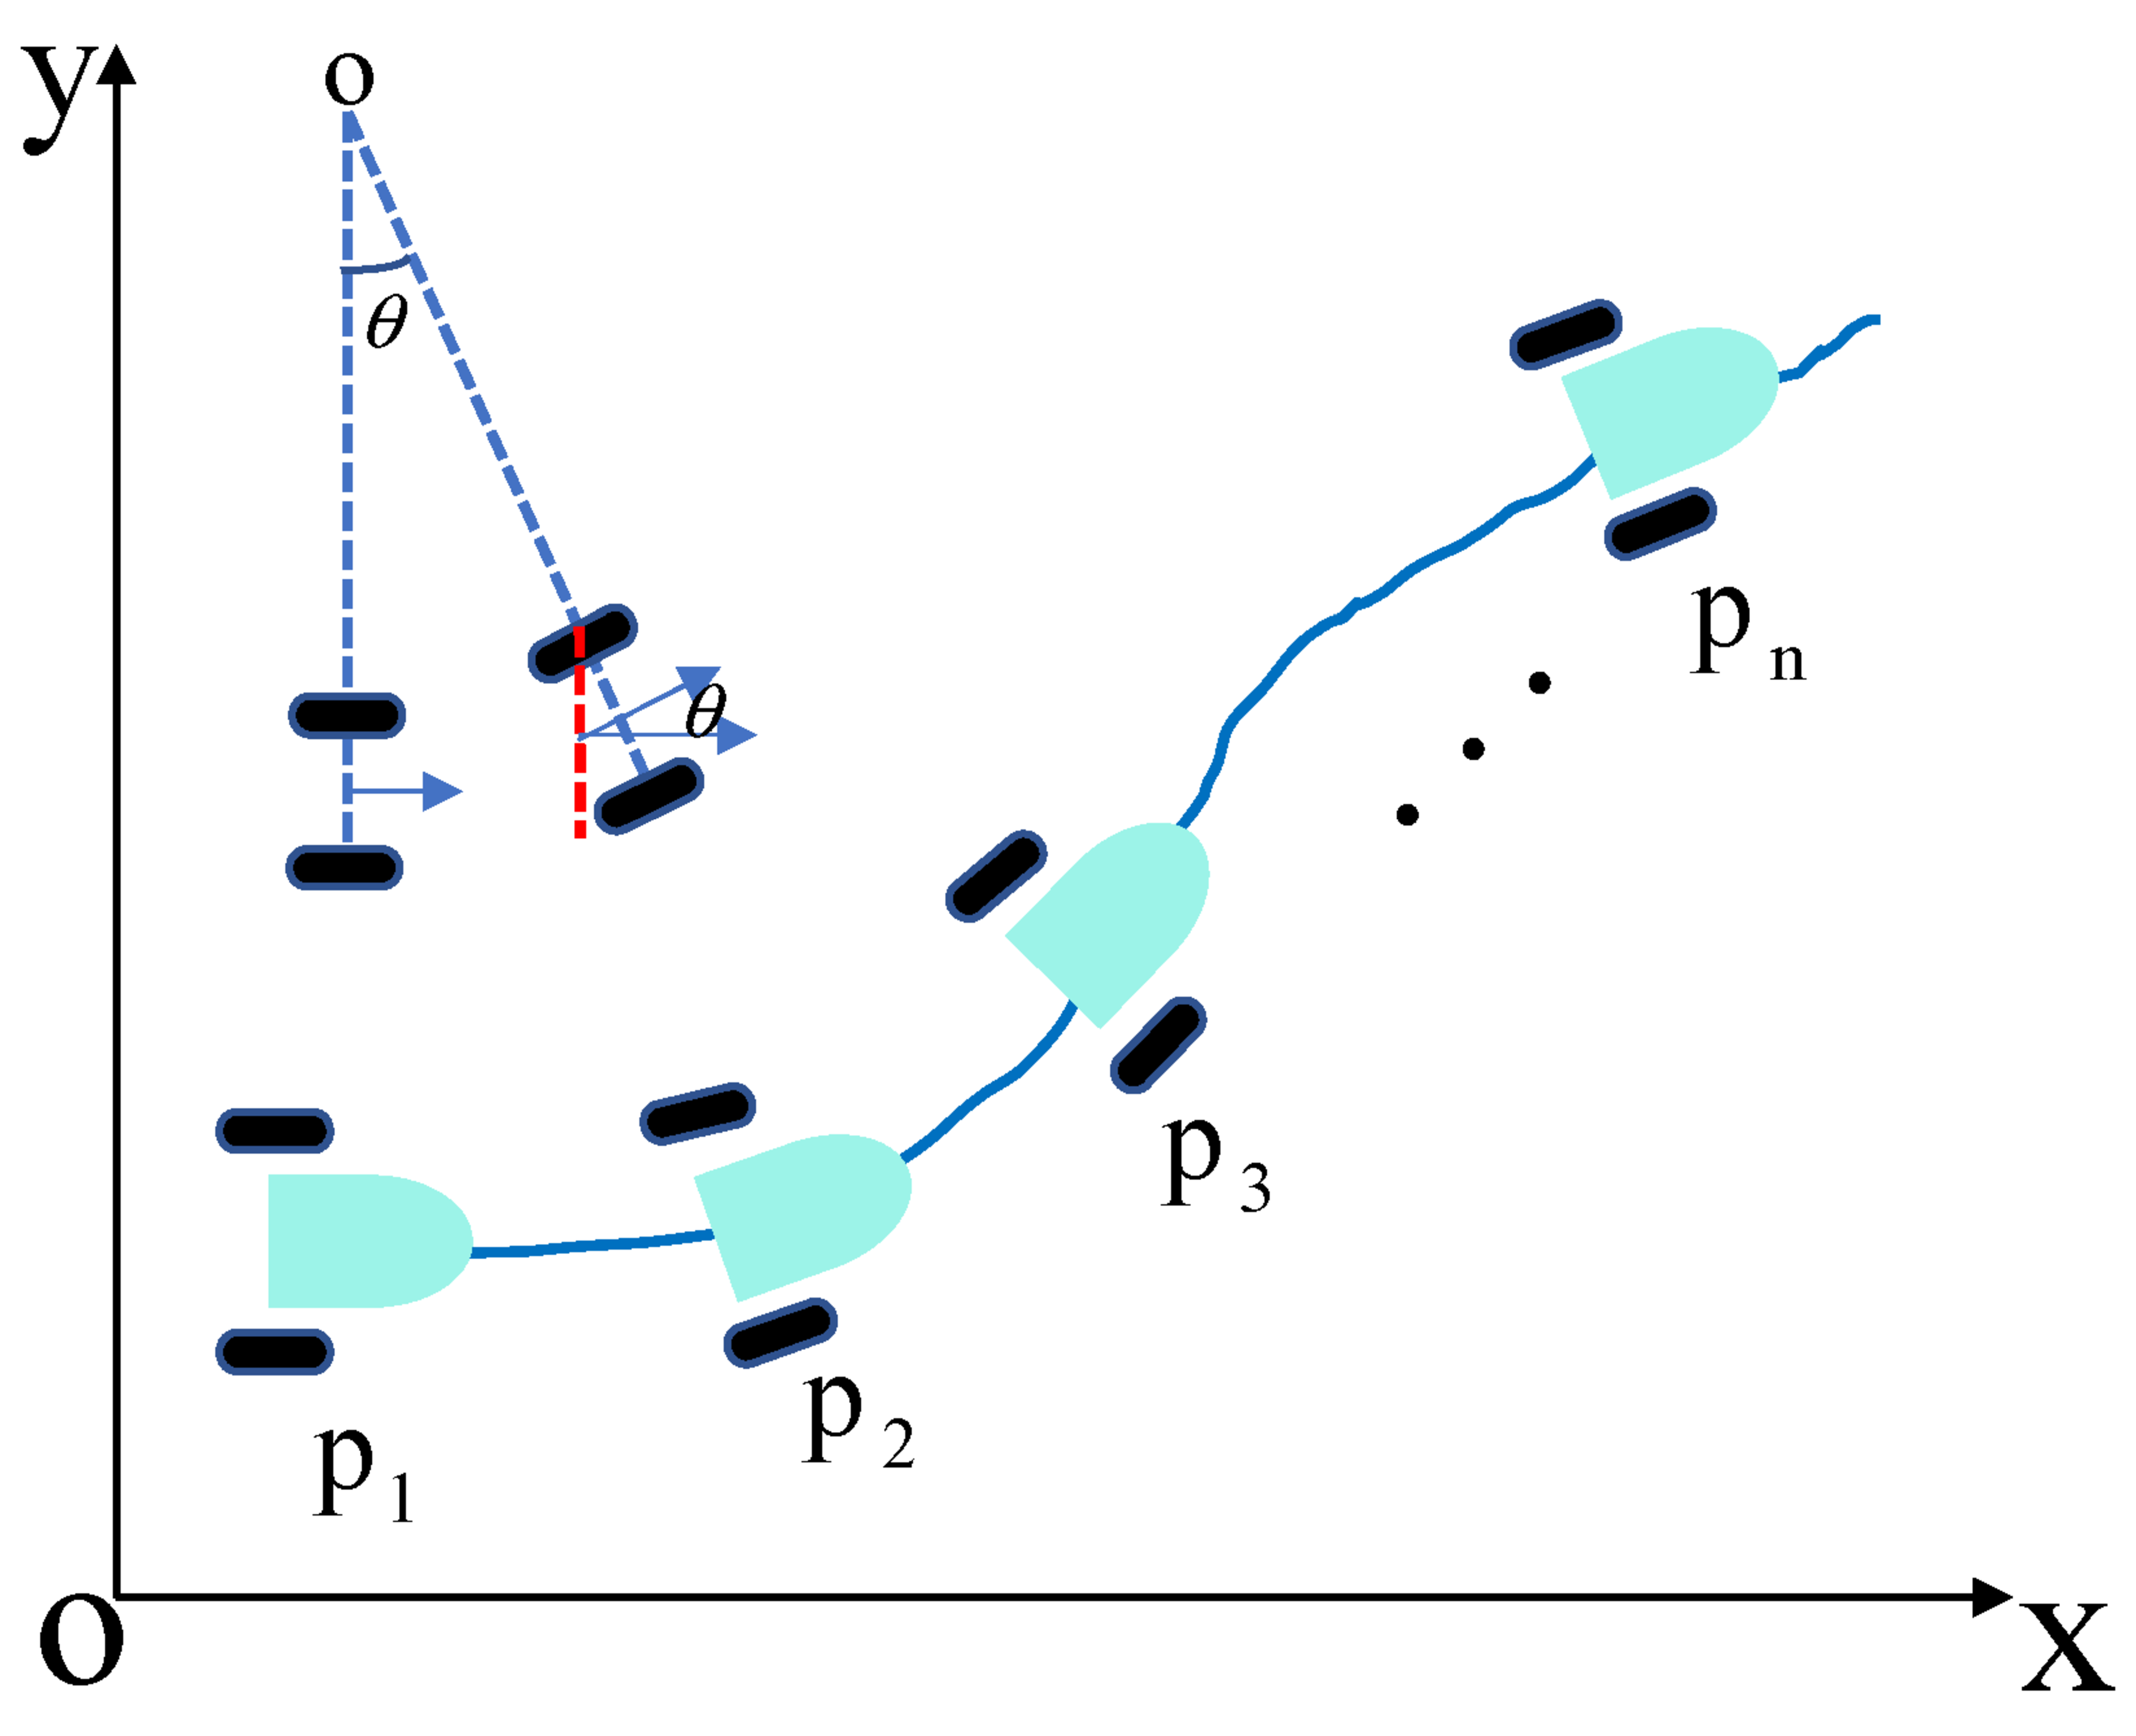
\includegraphics[width=0.5\textwidth]{deadreckoning.pdf} 
%     \caption{Dead Reckoning \cite{wei2022positioning}} 
%     \label{fig:deadreckoning} 
% \end{figure}

% While inertial navigation shares these conceptual roots, it leverages modern technology to measure motion far more precisely. 
% An INS relies on data from an Inertial Measurement Unit (IMU), which contains accelerometers to measure linear acceleration and gyroscopes to track angular rotation. 
% When an IMU's measurements are combined, they can reliably calculate a vehicle's position and orientation. 
% For instance, when a vehicle is traveling through a tunnel, GNSS signals are momentarily unavailable. 
% By combining the last known location obtained via GNSS with measurements captured by an IMU chip, a vehicle's movement can still be tracked during the GNSS outage, often with centimeter-level accuracy.
% Despite its advantages, INS has limitations, such as error accumulation over time due to the lack of external reference points, leading to drift in position estimates.
% To mitigate this, low-cost IMUs are primarily used to bridge periods when line-of-sight to satellites is obstructed.

% Inertial sensors are well suited for integration with GNSS systems owing to their
% complementary features.
% Unlike GNSS systems, the inertial navigation systems (INS) are self-contained and their
% performance is not degraded in environment as urban canyons, being independent of
% external electro-magnetic signals. Moreover INS are more accurate in the short term and
% they can supply data continuously with very high rate (at several hundred Hz, whereas
% GNSS receivers typically updates position and velocity at 1 to 20 Hz); INS can also
% provide attitude information.
% The main drawback of an INS is the degradation of its performance with time; in order
% to bound the errors to an acceptable level, regular updates are necessary and GNSS
% measurements can be used to this purpose.

%Stelzhammer
% As described by Werner [22], acceleration is the rate with which the speed of a mobile target changes relative to its own inertial frame. Based on smartphone acceleration, the current movement state of a device can be derived. For example, if no acceleration besides the earth’s gravitational pull, is experienced by the sensors, the device most probably is not moving.
% Acceleration is measured by observing the impact of acceleration onto a mass that is attached to a spring. The spring extends and contracts as the mass experiences accel- eration. The movement of the spring can be measured in order to derive an acceleration value. However, this construction has its downsides. Each measurement contains the earth’s gravitational force. Additional sensor have to be employed to correctly calculate the actual acceleration without the influence of the earth’s gravitational pull. Because of this, the orientation of the device is required in order to remove the constant earth accel- eration. Smartphones nowadays employ three basic accelerometers bundled together in a pairwise orthogonal manner. This enables smartphones to measure acceleration along three independent axes.
% In order to remove the earth’s acceleration from accelerometer measurements, a gy- roscope has to be utilized. As Werner [22] describes, a gyroscope measures rotational acceleration by exploiting the physical law of conservation of angular momentum. A rotating mass is mounted on rotational axes. If the device is tilted, the mass will cause the axes to rotate with respect to the tilt. The change in rotation of axes can be measured.
% Barometers are able to measure air pressure, as described by Werner [22], making it possible to calculate the height given the weather condition and vice versa. Applying the formula describing the relation between air pressure and height in standard weather criteria, the height difference in time can be calculated by taking measurements at different points in time. Taking ambient air pressure measurements in quick succession, the time can even be taken out of consideration.
% Most smartphones nowadays are equipped with barometers which makes it possible to utilize air pressure as contextual information in indoor navigation. With this approach it is possible to detect when the target is ascending or descending stairs by the air pressure sinking or rising respectively.
% Magnetometers are able to measure the magnetic flow in the environment, as stated by Werner [22]. Based on Hall sensors, the Hall effect is used to detect magnetic fields. If magnetic waves are flowing through the conductor inside the Hall sensor in orthogonal direction, the electrons are deflected from their straight path. This deflection of electrons causes one side of the conductor to become negatively charged whilst the other becomes positively charged. This leads to a measurable voltage between both sides of the sensor. By detecting such magnetic fields, a magnetometer is able to derive the magnetic north direction using the earth natural magnetic field. Nonetheless, the earth magnetic field is rather weak which makes it impossible to track the north direction accurately with a magnetic compass alone. A gyroscope is used to derive the additionally required information.

\section{Alerts on Smartphones}
Alert types, trigger conditions and restrictions define how and when users are notified of specific app events, ensuring that alerts provide value without disrupting user control. 
The following sections outline the types of alerts available, the mechanisms that trigger them and the specific guidelines imposed by Apple to maintain a responsible alert experience to users.

\subsection{Alert Types}
Smartphones offer different ways to alert users, including visual, sound and vibration cues. 
These alerts help confirm actions, share important information and improve user experience.
Notifications are one of the most common types of alerts and can be split into local and push notifications. 
According to Apple's documentation \cite{apple_local_notifications}\cite{apple_push_notifications}, local notifications are created by the app itself to inform users of events, even when the app runs in the background. 
Push notifications, sent from a server, are often used for real-time updates like messages or breaking news.
Another type of alert is haptic feedback, which uses vibrations to notify users physically. 
In iOS, tools like the UIImpactFeedbackGenerator provide vibrations for various levels of physical impact, such as light, medium or heavy taps.
The UISelectionFeedbackGenerator signals changes in selection, like scrolling through a picker, while the UINotificationFeedbackGenerator conveys success, warning or error notifications to clarify important feedback, as noted by the Apple Dev-Pages \cite{apple_haptics}.
Sound feedback is also available and is more noticeable, making it effective for capturing users' attention.
According to Apple's guidelines \cite{apple_sound_guidelines}, iOS sounds are divided into system sounds, used for standard actions like errors or confirmations and custom sounds, often used in games or specific app events to create unique auditory experiences.
For visual feedback, Apple's UIAlertController \cite{apple_alerts} provides pop-up alerts with titles, messages and action buttons, often used for critical alerts or confirmations to ensure user attention. 
Toasts, which are brief messages that appear and disappear without user interaction, are another form of visual feedback. 
While not native to iOS, third-party frameworks can enable toasts, offering a less intrusive way to share short information. 
Subtler visual cues, like progress indicators and badges, are also effective for showing ongoing tasks or highlighting unread notifications within app sections.
With iOS 16, Apple introduced the Live Activities feature \cite{apple_live_activities}, which displays real-time updates on the lock screen or in the Dynamic Island. 
This feature keeps users informed about ongoing events, such as tracking a food delivery or monitoring live sports scores, without needing to open the app.

\subsection{Triggers}
In iOS, alerts are not limited to user input, they can also be triggered by automated or event-based conditions. 
Apps, for example, can use scheduled timers to generate alerts or notifications at specific times for reminders, countdowns or periodic updates. 
This is often implemented using Swift's Timer class \cite{apple_timer}.
Alerts can also respond to app state changes, such as when an app transitions to the background, returns to the foreground or closes. 
For instance, an app may display a confirmation alert if the user attempts to leave a page with unsaved data or notify them of an important update using UIApplicationDelegate \cite{apple_app_delegate}.
Device sensors like accelerometers and gyroscopes detect motion or orientation changes, which can also trigger alerts.
Location-based triggers, which are central to this thesis, use geographical boundaries to deliver alerts when a user moves into or out of a specified region.
Apple's CoreLocation framework provides tools like CLLocationManager for managing these triggers, while CoreMotion supports motion event detection \cite{apple_corelocation, apple_coremotion}. 
Similarly, HealthKit \cite{apple_healthkit} enables alerts based on health metrics, such as notifying users if their heart rate exceeds a specified threshold.
To manage in-app notifications, Apple's NotificationCenter is frequently used to broadcast data changes, enabling observers to update alerts or badges in real time \cite{apple_notificationcenter}. 
For notifications, iOS provides three main trigger types. 
UNTimeIntervalNotificationTrigger \cite{apple_time_trigger} schedules alerts after a specified time interval. 
UNCalendarNotificationTrigger \cite{apple_calender_trigger} triggers notifications at specific dates or times, with options for recurring alerts and UNLocationNotificationTrigger \cite{apple_location_trigger} sends alerts when a user enters or leaves predefined geographical areas.

\subsection{Restrictions in iOS}
When it comes to responsible app development, Apple has many guidelines to maintain user control, ensure privacy and prevent disruptive app behavior. 
Generally, apps are restricted from triggering alarms or alerts when not actively running in the foreground, with exceptions for specific cases like Voice over IP (VoIP), music streaming and location-tracking apps. 
These applications can run background audio, but this capability is not intended for alarms and comes with strict guidelines to prevent misuse. 
For instance, while a music app may play in the background, an alarm app that attempts to exploit this mode to ring an alarm would be rejected. 
This limitation makes it challenging to release an app that plays sounds solely for alerts, though this is not the goal of this thesis.
Additionally, iOS does not provide any public API for third-party apps to set, modify or access alarms in the native Clock app, which is entirely separate and inaccessible for tasks like scheduling alarms or timers. 
When delivering notifications, apps must obtain user permission. 
Users can choose to allow, mute or disable notifications from each app, and Apple discourages excessive notifications, especially those lacking immediate or relevant value. 
Apps that send spammy notifications risk penalties or even removal from the App Store. 
Custom sounds for local notifications are limited to 30 seconds, if a sound exceeds this limit, iOS defaults to the standard notification sound, as discussed on the Apple Developer website \cite{apple_sound_guidelines}.
Local notifications also respect Silent Mode and Do Not Disturb settings, meaning sounds will not play if these modes are active. 
According to Apple's documentation \cite{apple_critical_alerts}, critical alerts are allowed to bypass these settings, but this permission is reserved for essential use cases, such as health monitoring or emergency alerts, not for general alarms or reminders. 
Location-based triggers, such as geofencing, also require explicit user permission. 
IOS \cite{apple_geofencing_limits} limits the frequency of location-based notifications and may throttle frequent triggers. 
Excessive location tracking can lead to App Store rejection unless it is essential to the app's function. 
Additionally, Apple restricts the use of geofencing to a maximum of 20 active geofences per app to conserve battery life and optimize performance. 

\section{Geofencing}
% Shevchenko and Reips \cite{shevchenko2024geofencing} define geofencing as the automated triggering of actions when "virtual boundaries around specific locations" are crossed. It relies on multiple location-based technologies, including GNSS, Wi-Fi, and cellular networks, to establish and monitor these predefined geographic boundaries. Over time, it has become a useful tool with applications across different industries.

% Geofencing enhances user experiences by providing personalized services, such as sending targeted advertisements or adjusting smart home settings when people enter or leave specific areas. It is also widely used in business operations, including logistics, healthcare and workforce management, where it helps streamline processes and improve efficiency. However, as Greenwald \cite{greenwald2011geofencing} highlights, geofencing raises significant concerns, particularly regarding privacy. Since it relies on continuous location tracking, users' sensitive data may be vulnerable to misuse or security breaches, especially when the technology overlaps with personal or sensitive areas such as homes or healthcare facilities.

% Initially designed for military and government use in the 1990s, geofencing has since expanded into a variety of domains due to advancements in GPS-enabled smartphones and mobile technologies \cite{westbrook2019gps}. In marketing, for instance, businesses use geofencing to send location-based advertisements or discounts to customers near their stores, creating personalized shopping experiences and increasing sales \cite{greenwald2011geofencing}. Workforce management benefits from geofencing by automating employee attendance tracking, where staff can clock in and out automatically upon entering or leaving work zones, reducing manual errors and administrative burdens \cite{amudha2019smarthome}.
% Geofencing is also transforming home automation in the Internet of Things (IoT) domain. For example, smart devices can adjust lighting, heating, or security systems based on residents' proximity to their homes \cite{amudha2019smarthome}. Similarly, it has proven valuable in agriculture, where geofencing combined with IoT helps protect crops from wild animal intrusions by sending farmers real-time alerts to minimize damage \cite{kadam2020crops}. In educational settings, Takyiwa-Debrah \cite{takyiwa2023geofence} highlights how geofencing improves child safety by integrating GPS-enabled wearable devices, which provide real-time location tracking to prevent abductions in schools.
% In logistics, geofencing ensures vehicles adhere to designated routes and allows businesses to monitor fleet locations in real time, improving efficiency and security \cite{reclus2009fleet}. In healthcare, it helps caregivers monitor dementia patients by setting up safe zones and alerting them when patients move beyond these boundaries, enabling prompt interventions and ensuring patient safety \cite{arora2023location}.

\section{Converting Speech to Text}
% WRITE HOW STT IS USED IN THE APP; SET UP REMINDERS WITH VOICE-CONTROL
% Speech-to-text (STT) is a technology that turns spoken words into written text. It works by listening to audio and using voice recognition to understand and transcribe the words. The result is a text document that captures what was said. While speaking is the most natural and efficient way to communicate, audio recordings alone can be difficult to review or reuse quickly. This makes speech-to-text an essential tool across many fields. For instance, it enables record-keeping of patient notes in healthcare or court proceedings in legal services, supports transcription of lectures in education, streamlines workflows in media and customer service by converting interviews or calls into text. Furthermore, it is widely used in virtual assistants to process voice commands, as well as in closed captioning to make videos accessible to broader audiences. It also plays a key role in creating accessibility tools for individuals with hearing impairments.

% Rabiner and Juang \cite{rabiner1993speechrecognition} explain that speech can be understood as an audio signal characterized by its frequency, amplitude and temporal patterns, which define the unique qualities of spoken language. They further emphasize that speech is made up of different components that work together to create meaning and structure. One of the most basic elements is phonemes, which are the smallest units of sound in a language, like the "b" in "bat". These phonemes combine to form syllables, which are the building blocks of words, such as "bat" having one syllable and "better" having two. Beyond these, intonation patterns refer to the rise and fall of pitch in speech, which help convey emotions, emphasis or the difference between a question and a statement. According to Reetz \cite{reetz2020phonetics}, the process of turning speech into text depends on acoustic properties and linguistic understanding. Acoustic models focus on the sound itself, breaking down the audio into patterns like pitch, tone and duration to identify specific sounds or words. Meanwhile, language models go a step further by applying rules of grammar, vocabulary and sentence structure to make sense of those sounds in context. Together, these models ensure that the transcription is not only accurate in identifying the sounds but also meaningful and grammatically correct in written form.

% However, speech-to-text faces several challenges that can impact its accuracy. Background noise, such as conversations, traffic or music, can interfere with speech clarity and make transcription difficult. Regional accents and dialects add variability in pronunciation, which can lead to misinterpretations. Additionally, Zechner and Waibel \cite{zechner20000spontaeousspeech} highlight that conversations with multiple speakers, especially when voices overlap, present difficulties in separating speech accurately. Spontaneous speech, with its non-standard grammar, fillers like "um" or "uh," and frequent self-corrections, further complicates transcription, as stated by Furiu et al. \cite{furiu2004spontaneousspeech}. Lastly, technical vocabulary can be challenging for the system to recognize without prior training.

% In Fig.~\ref{fig:stt_pipeline} by Rabiner and Juang \cite{rabiner1993speechrecognition}  the speech-to-text pipeline is illustrated by breaking down the process into different stages, starting with signal processing, where speech is captured and analyzed to differentiate between voiced, unvoiced and silent segments. Next, feature extraction transforms the raw audio into meaningful data points, which are then segmented into smaller units for easier processing. The labeling and sound merging steps classify individual sounds and combine them into coherent units, guided by sound classification and phonotactic rules. Sound classification identifies sounds, such as vowels or consonants, based on their unique acoustic patterns, while phonotactic rules ensure that recognized sounds follow the natural language patterns, enhancing transcription accuracy.  Word verification and sentence verification ensure the transcription is contextually meaningful by leveraging lexical access and language models. Throughout the pipeline, knowledge sources such as phonotactic rules and linguistic models play an important role in improving the transcription and producing a recognized utterance.

% \begin{figure}[htbp]
%     \centering
%     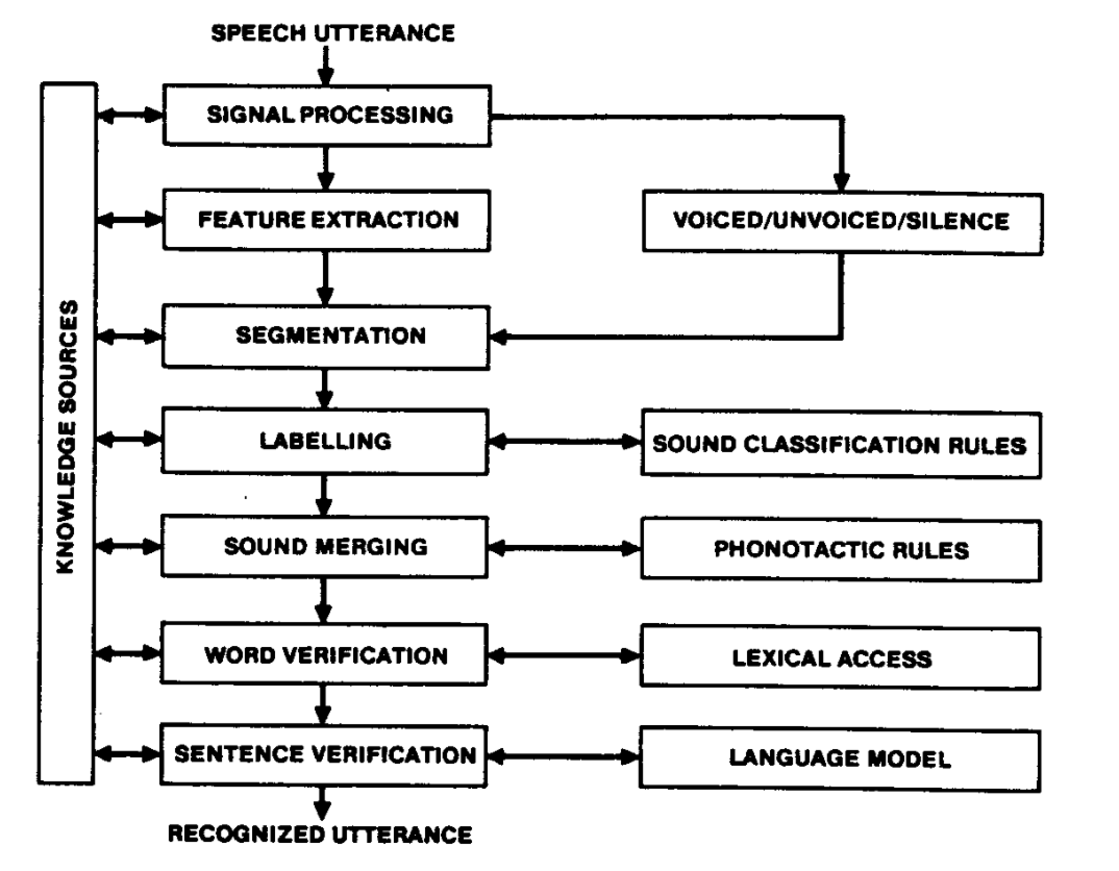
\includegraphics[width=0.7\textwidth]{stt_pipeline.pdf}
%     \caption{Knowledge integration in speech recognition \cite{rabiner1993speechrecognition}}
%     \label{fig:stt_pipeline}
% \end{figure}

\section{Large Language Models}
% WRITE HOW LLM IS USED IN THE APP; PARSING STT TRANSCRIPT TO CERTAIN FORMAT TO DISTINGUISH WHICH START, STOP STATION, MODE, INTERVAL
% large language models, was ist, welche gibts, wieso chat gpt api??
% \chapter{Related Work}
\label{cha:RelatedWork}

\section{Google Maps}
\section{Citymapper}
\section{Moovit}
\section{Transit}

\chapter{Concept}
\label{cha:Concept}

\section{Overview}

\section{Types of Alert Systems}
\subsection{Time-Based Mode}
% Scheduling Alerts Based on Specific Times

\subsection{Station-Based Mode}
% Monitoring Stations Using Geofences

\subsection{Distance-Based Mode}
% Nesting Geofence Regions Around the Destination

% \section{Alerts on Smartphones}
% For the implementation of a user-focused alert app in public transportation that ensures the passengers get reminded when to get off in an effective manner, notifications only aren't sufficient enough. So, this app will support vibrations and alarms as well as notifications. 

% \subsection{Alert Types}
% The primary users of the alert app are passengers in public transportation, where it is common for people to travel alongside others in shared spaces. In this setting, it's important to alert users effectively while avoiding disruption to other passengers. To address this need, the app incorporates a tiered system of three escalating alert types. These alert types range from minimally intrusive notifications to highly noticeable alarms, allowing users to select their preferred alert level.
% This tiered approach ensures that users receive the necessary alerts without causing undue disruption, enhancing both user experience and public courtesy.

% When a user approaches their designated stop, the app's first alert is always a notification, as it is the least intrusive option. This notification is mandatory and cannot be disabled by the user. However, certain device settings, such as silent mode, can reduce its effectiveness by muting audible cues. Additionally, by default push notifications aren't being displayed when an app is in the foreground state. Now users may wish to monitor their location on the map, which would prevent visual notifications unless the app is in the background. But this can be addressed programmatically, as discussed further in Chapter 5.
% Therefore, notifications alone are sufficient only when users have their device in hand and are able to see or hear the alert.

% Building on the limitations of notifications, the app's second alert is vibration, which users can select if preferred. Vibration provides a moderately more noticeable alert without disturbing other passengers, as it is silent. This option is particularly useful if the phone is in silent mode or if the user is distracted and it functions if the app's in both the foreground and background.
% However, vibrations alone may still be insufficient in certain cases. For example, if the user is asleep, or if the phone is stored in a bag where the vibration may not be felt, the alert might go unnoticed. Additionally, since the vibration is not accompanied by a visual cue, users may forget they set a reminder or may mistake the vibration for a different type of alert.

% Finally, for cases where the user may be asleep or highly distracted, the app provides an audible alarm designed to capture the user's full attention as a third alert option. Due to its intrusive nature, this alert may be disruptive to nearby passengers. The alarm can be silenced by pressing the volume controls or by using a designated button in the app's reminder overview, which becomes available while the alarm is active.

% \subsection{Triggers}
% In the app the user can choose the interval in which he/she wants to receive the notification, the triggers of the vibration and alarm cannot be altered by the user. But depending on the preferred trigger type, the user can choose over three modes which are different in the triggers that activate the alerts. There is a time-based mode which uses the scheduled arrival times of public transportation and calculates the trigger time according to the estimated stop arrival time. The user can choose between wanting to receive a notification 5, 7 or 10 minutes before arrival. The vibration will happen 3 minutes before and the alarm 2 minutes. As for the staion-based mode, it uses three geofences along the route to progressively alert the user. The notification can be scheduled for 3, 4 or 5 stations before, the vibration is 2 stations before and the alarm 1. The last mode is the distance mode which relies on nested geofences around the final destination to trigger alerts. The user can choose to receive the notification 500, 750 meters, 1, 1.5 or 2 kilometers before, the vibration is 350 meters before and the alarm 250 meters.
\chapter{Implementation}
\label{cha:Implementation}

\section{System Architecture}
\section{UI Prototypes}
\section{Storing and Accessing User Data}

\section{iOS GeofenceManager using CLLocationManager}
% entering region once and alarm sounds or notification is sent and then leaving region and reentering
%https://developer.apple.com/documentation/corelocation/cllocationmanager
%https://developer.apple.com/documentation/CoreLocation
\subsection{Permissions and Capabilities}
\subsection{Start Monitoring Region}
\subsubsection{Geofence Level 1: Notification}
\subsubsection{Geofence Level 2: Vibration}
\subsubsection{Geofence Level 3: Alarm}
\subsection{Stop Monitoring Region}

\section{Notification Management in iOS}
\subsection{Permissions and Capabilities}
\subsection{Scheduling Notifications Locally}

\section{Alarm Management in iOS}

\section{Displaying Routes on Map}

\section{Simulation of Routes}

\section{Voice-Controlled Alert Setup}
\subsection{Transcribing Speech to Text}
\subsection{Generating AI Response from Speech and Prompt}
\subsection{Scheduling Alert}

\chapter{Conclusion}
\label{cha:Conclusion}

\section{Resume}

\section{Next Steps}

%%%-----------------------------------------------------------------------------
\appendix                                                             % Appendix 
%%%-----------------------------------------------------------------------------

\chapter{Acronyms}
\label{app:Acronyms}

\begin{acronym}[XXXX] % [XXXX] sets the width for the longest acronym
    \acro{API}{Application Programming Interface}
    \acro{APs}{Access Points}
    \acro{AoA}{Angle of Arrival}
    \acro{A-GPS}{Assisted GPS}
    \acro{BLE}{Bluetooth Low Energy}
    \acro{CoO}{Cell of Origin}
    \acro{CPS}{Cellular Positioning System}
    \acro{DoA}{Direction of Arrival}
    \acro{DoD}{Department of Defense}
    \acro{E-911}{Enhanced 911}
    \acro{E-OTD}{Enhanced Observed Time Difference}
    \acro{FCC}{Federal Communications Commission}
    \acro{GNSS}{Global Navigation Satellite System}
    \acro{GPS}{Global Positioning System}
    \acro{GSM}{Global System for Mobile Communications}
    \acro{IMU}{Inertial Measurement Unit}
    \acro{INS}{Inertial Navigation System}
    \acro{IoT}{Internet of Things}
    \acro{IPS}{Indoor Positioning Systems}
    \acro{LBS}{Location-Based Services}
    \acro{LMUs}{Location Measurement Units}
    \acro{LTE}{Long Term Evolution}
    \acro{PSAPs}{Public Safety Answering Points}
    \acro{RFID}{Radio Frequency Identification}
    \acro{RSS}{Received Signal Strengths}
    \acro{RSSI}{Received Signal Strength Indicator}
    \acro{SNR}{Signal-to-Noise Ratio}
    \acro{STT}{Speech-to-Text}
    \acro{ToA}{Time of Arrival}
    \acro{TDoA}{Time Difference of Arrival}
    \acro{TTFF}{Time to First Fix}
    \acro{UI}{User Interface}
    \acro{UMTS}{Universal Mobile Telecommunications System}
    \acro{U-TDoA}{Uplink Time Difference of Arrival}
    \acro{UUID}{Universally Unique Identifier}
    \acro{UWB}{Ultra-Wideband}
    \acro{Wi-Fi}{Wireless Fidelity}
    \acro{WPS}{Wi-Fi-based Positioning Systems}
    \acro{WLAN}{Wireless Local Area Network}
    \acro{5G}{5th Generation}
\end{acronym} % Acronyms
% \chapter{Supplementary Materials}
\label{app:materials}


List of supplementary data submitted to the degree-granting institution for archival storage
(in ZIP format).

% Use this as an example only, adapt the structure to your requirements!

% \section{PDF Files}
% \begin{FileList}{/}
% \fitem{thesis.pdf} Master/Bachelor thesis (complete document)
% \end{FileList}

% \section{Media Files}
% \begin{FileList}{/media}
% \fitem{*.ai, *.pdf} Adobe Illustrator files
% \fitem{*.jpg, *.png} raster images
% \fitem{*.mp3} audio files
% \fitem{*.mp4} video files
% \end{FileList}

\section{Source Code}

\section{Online Sources (PDF Captures)}
\begin{FileList}{/online-sources}
\fitem{Reliquienschrein-Wikipedia.pdf} {\backtrackerfalse\parencite{WikiReliquienschrein2023}}
\end{FileList}




 % Contents of the CD-ROM/DVD
% \include{back/appendix_c} % Chronological list of changes
% \include{back/appendix_d} % Source text of this document

%%%-----------------------------------------------------------------------------
\backmatter                           % Back part (bibliography, glossary, etc.)
%%%-----------------------------------------------------------------------------

\MakeBibliography % References

%%%-----------------------------------------------------------------------------
% Special page for checking print size
%%%-----------------------------------------------------------------------------

\include{back/printbox}

%%%-----------------------------------------------------------------------------
\end{document}
%%%-----------------------------------------------------------------------------
